\newcommand*{\INVERTED}{} % Comment out for light-mode
\newcommand*{\CENTERTITLE}{} % Comment out for left-aligned title

\usepackage{fontspec}
\usepackage{sourcesanspro}
\usepackage[T1]{fontenc}

% NOTE: You will need to pull this code via the GitHub repo and compile with latexmk
% to get new pythontex syntax highlighting working properly.
% \documentclass[aspectratio=169]{beamer-pytex}

\setbeamertemplate{title page}[default][left] % left-align title page (commend out for centered title page)
\beamertemplatenavigationsymbolsempty % remove navigation symbols

\newcommand*{\INVERTED}{} % Comment out for light-mode
\newcommand*{\CENTERTITLE}{} % Comment out for left-aligned title

\usepackage{fontspec}
\usepackage{sourcesanspro}
\usepackage[T1]{fontenc}

\usepackage[usefamily={jl,julia,juliacon}]{pythontex}
\setpythontexpygopt{style=algfordm}

% NOTE: You will need to pull this code via the GitHub repo and compile with latexmk
% to get new pythontex syntax highlighting working properly.
\documentclass[aspectratio=169]{beamer-pytex}

\setbeamertemplate{title page}[default][left] % left-align title page (commend out for centered title page)
\beamertemplatenavigationsymbolsempty % remove navigation symbols

\input{preamble}

\title{\texttt{Julia in Academia}}
\subtitle{Textbooks, Stanford Courses, and the Future}
\author{Robert Moss, PhD}
\institute{Stanford University | JuliaCon 2025}
\email{mossr@cs.stanford.edu}
\date{}

\begin{document}

\begin{frame}
    \maketitle
\end{frame}

\include{slides/whoami}
\include{slides/textbooks}
\include{slides/textbooks-juliacon-2019}
\include{slides/textbooks-julia}
\include{slides/textbooks-julia-code}
\include{slides/textbooks-julia-code-repo}
\include{slides/julia-slides-repo}
\include{slides/integrated-julia}
\include{slides/textbooks-the-good}
\include{slides/integrated-showcase}
\include{slides/textbooks-the-not-so-good}
\include{slides/stanford-courses}
\include{slides/stanford-courses-lectures}
\include{slides/stanford-courses-lectures-pluto}
\include{slides/pluto-assignments}
\include{slides/grading-assignments}
\include{slides/future}
\include{slides/plutopapers}
\include{slides/questions}

\end{document}

% TODO: albatian
\usefonttheme{serif}
\usefonttheme{professionalfonts}
\usepackage{mathtools}
\usepackage[tracking=true]{microtype}

\usepackage{bold-extra}
\usepackage{realscripts}
\usepackage{amsmath,bm,amssymb}
\usepackage{amsthm}
\usepackage{bbm}
\usepackage{tikz}
\usepackage[group-digits=integer,group-minimum-digits=4,group-separator={,},detect-all]{siunitx}
\usepackage{algorithmicx}
\usepackage{algorithm}
\usepackage[noend]{algpseudocode}
\usepackage{textpos}
\usepackage{xcolor}
\usepackage{multirow}
\usepackage{longtable,tabularx,booktabs}
\usepackage[flushleft]{threeparttable}
\usepackage{vector} % local
\usepackage{varwidth}
\usepackage{fancyvrb}
\usepackage{tcolorbox}
\usepackage{ifthen}

%%%%%%%%%%%%%%%%%%%%%%%%%%%%%%%%%%%%%%%%%%%%%%%%%%
% Unicode settings
%%%%%%%%%%%%%%%%%%%%%%%%%%%%%%%%%%%%%%%%%%%%%%%%%%
\setmonofont{DejaVu Sans Mono}[Scale=MatchLowercase]
\usepackage{newunicodechar}
\newfontface{\calligraphic}{Latin Modern Math}[Scale=0.85]


%%%%%%%%%%%%%%%%%%%%%%%%%%%%%%%%%%%%%%%%%%%%%%%%%%
% Reference (biber) settings
%%%%%%%%%%%%%%%%%%%%%%%%%%%%%%%%%%%%%%%%%%%%%%%%%%
\usepackage[style=verbose,backend=biber]{biblatex}
% \addbibresource{preamble/main.bib}
\addbibresource{\jobname.bib}
% \setbeamerfont{footnote}{size=\tiny}
\setbeamerfont{footnote}{size=\fontsize{4}{5}\selectfont}
\setbeamertemplate{bibliography item}{}% Remove reference icon.
\renewcommand*{\bibfont}{\footnotesize}


%%%%%%%%%%%%%%%%%%%%%%%%%%%%%%%%%%%%%%%%%%%%%%%%%%
% Colors
%%%%%%%%%%%%%%%%%%%%%%%%%%%%%%%%%%%%%%%%%%%%%%%%%%
\ifdefined\INVERTED
    \colorlet{primarycolor}{white}
    \colorlet{secondarycolor}{black}
    \colorlet{shadecolor}{black!85}
    \definecolor{cardinal}{HTML}{B83A4B}
    \definecolor{coolgrey}{HTML}{767674}
    \definecolor{captioncolor}{HTML}{59B3A9}
    \definecolor{captionsecondarycolor}{HTML}{2D716F}
    \colorlet{pagecolor}{lightgray}
    \colorlet{algbgcolor}{darkgray}
\else
    \colorlet{primarycolor}{black}
    \colorlet{secondarycolor}{white}
    \colorlet{shadecolor}{black!5}
    \definecolor{cardinal}{HTML}{8C1515}
    \definecolor{coolgrey}{HTML}{53565A}
    % \definecolor{captioncolor}{HTML}{3333B2} % Blue
    % \definecolor{captionsecondarycolor}{HTML}{7A7ACD} % Light blue
    \definecolor{captioncolor}{HTML}{59B3A9}
    \definecolor{captionsecondarycolor}{HTML}{2D716F}
    \colorlet{pagecolor}{darkgray}
    \colorlet{algbgcolor}{lightgray}
\fi

\definecolor{darkgreen}{RGB}{21,140,21}
\definecolor{darkblue}{RGB}{21,21,140}
\definecolor{sun}{RGB}{234,171,0}

\newcommand{\darkblue}[1]{{\color{darkblue} #1}}
\newcommand{\darkgreen}[1]{{\color{darkgreen} #1}}
\newcommand{\darkred}[1]{{\color{cardinal} #1}}

\definecolor{pastelMagenta}{HTML}{FF48CF}
\definecolor{pastelPurple}{HTML}{8770FE}
\definecolor{pastelBlue}{HTML}{1BA1EA}
\definecolor{pastelSeaGreen}{HTML}{14B57F}
\definecolor{pastelGreen}{HTML}{3EAA0D}
\definecolor{pastelOrange}{HTML}{C38D09}
\definecolor{pastelRed}{HTML}{F5615C}

% \begin{jlcode}
%     include("../../jl/support_code.jl")

%     using Colors
%     using ColorSchemes
%     pasteljet = ColorMaps.RGBArrayMap(ColorSchemes.viridis, interpolation_levels=500, invert=true);
%     pastelRedBlue = ColorMaps.RGBArrayMap([RGB(246/255, 21/255, 92/255),
%                                            RGB(1.0,1.0,1.0),
%                                            RGB( 27/255,161/255,234/255)], interpolation_levels=500);
% \end{jlcode}


%%%%%%%%%%%%%%%%%%%%%%%%%%%%%%%%%%%%%%%%%%%%%%%%%%
% PGFPlot settings
%%%%%%%%%%%%%%%%%%%%%%%%%%%%%%%%%%%%%%%%%%%%%%%%%%
% \usepackage[pgfplots]{../juliaplots.sty/juliaplots}
\usepackage{pgfplots}
\pgfplotsset{compat=newest}
\pgfplotsset{every axis legend/.append style={legend cell align=left, font=\footnotesize, draw=none, fill=none}}
\pgfplotsset{every axis/.append style={axis background/.style={fill=secondarycolor}}}
\pgfplotsset{every tick label/.append style={font=\footnotesize}}
\pgfplotsset{every axis label/.append style={font=\footnotesize}}

\fvset{baselinestretch=0.8}
\usepgfplotslibrary{fillbetween}
\usepgfplotslibrary{groupplots}
\usepgfplotslibrary{patchplots}
\usepgfplotslibrary{statistics}
\usepgfplotslibrary{ternary}


%%%%%%%%%%%%%%%%%%%%%%%%%%%%%%%%%%%%%%%%%%%%%%%%%%
% TikZ settings
%%%%%%%%%%%%%%%%%%%%%%%%%%%%%%%%%%%%%%%%%%%%%%%%%%
\usetikzlibrary{calc}
\usetikzlibrary{fit}
\usetikzlibrary{positioning}
\usetikzlibrary{arrows}
\usetikzlibrary{arrows.meta}
\usetikzlibrary{decorations.pathreplacing}
\usetikzlibrary{decorations.pathmorphing}
\usetikzlibrary{decorations.text}
\usetikzlibrary{patterns}
\usetikzlibrary{graphs}
\usetikzlibrary{graphdrawing}
\usetikzlibrary{shapes}

\tikzset{
    func/.style = {rectangle, rounded corners=1, draw},
    partial/.style = {rectangle, darkgreen, font=\bfseries},
    input/.style = {rectangle},
    nnnode/.style = {circle, draw=primarycolor, fill=secondarycolor, minimum size=16pt,},
}

\tikzstyle{solid_line}=[solid, thick, mark=none]
\tikzset{every picture/.style={semithick, >=stealth'}}
\tikzset{myline/.style={line width = 0.05cm, rounded corners=5mm}}
\tikzset{myarrow/.style={line width = 0.05cm, ->, rounded corners=5mm}}
\tikzset{myaxis/.style={thick, ->, line cap=rect}}
\tikzset{roundednode/.style={rounded corners=4mm,draw=primarycolor,fill=secondarycolor,line width=0.05cm, minimum size=0.35in, align=center}}



%%%%%%%%%%%%%%%%%%%%%%%%%%%%%%%%%%%%%%%%%%%%%%%%%%
% Custom commands
%%%%%%%%%%%%%%%%%%%%%%%%%%%%%%%%%%%%%%%%%%%%%%%%%%
\newcommand{\smallcaps}[1]{\textsc{#1}}

\usepackage{mdframed}
\newenvironment{algorithmblock}[1][htbp]
{\begin{mdframed}[backgroundcolor=shadecolor,fontcolor=primarycolor,linecolor=primarycolor,rightline=false,leftline=false]}
{\end{mdframed}}

\newenvironment{definitionblock}[1]{%
    \begin{mdframed}[backgroundcolor=shadecolor,fontcolor=primarycolor,linecolor=primarycolor,rightline=false,leftline=false]
        \textbf{Definition: #1.}\;
}{%
    \end{mdframed}
}

\newenvironment{centerjuliaverbatim}{%
  \par
  \centering
  \varwidth{\linewidth}%
  \juliaverbatim
}{%
  \endjuliaverbatim
  \endvarwidth
  \par
}


%%%%%%%%%%%%%%%%%%%%%%%%%%%%%%%%%%%%%%%%%%%%%%%%%%
% Beamer settings
%%%%%%%%%%%%%%%%%%%%%%%%%%%%%%%%%%%%%%%%%%%%%%%%%%
\addtobeamertemplate{navigation symbols}{}{%
    % Page numbers
    \usebeamerfont{footline}%
    \usebeamercolor[fg]{footline}%
    \hspace{1em}%
    \insertframenumber/\inserttotalframenumber
}

\newcommand{\email}[1]{\def\@email{\texttt{\MakeLowercase{\textls[10]{#1}}}}}

\setbeamercolor{background canvas}{bg=secondarycolor} % Set background color
\setbeamercolor{normal text}{fg=primarycolor}       % Set foreground color

% \setbeamerfont{title}{series=\bfseries} % family=\sourcesanspro
\setbeamercolor{title}{fg=secondarycolor}
\setbeamerfont{subtitle}{series=\scshape} % family=\sourcesanspro
\setbeamercolor{subtitle}{fg=primarycolor}
\setbeamerfont{author}{series=\scshape,family=\sourcesanspro}
\setbeamercolor{author}{fg=primarycolor}
\setbeamerfont{institute}{series=\scshape}
\setbeamercolor{institute}{fg=cardinal}
\setbeamercolor{email}{fg=coolgrey}
\setbeamerfont{date}{family=\sourcesanspro,series=\scshape,size=\tiny}
\setbeamercolor{date}{fg=coolgrey}

\setbeamercolor{bibliography entry author}{fg=captioncolor} % Set author names
\setbeamercolor{bibliography entry note}{fg=captionsecondarycolor} % Set journal/publisher

\setbeamercolor{footline}{fg=pagecolor} % Page number color

\setbeamercolor{caption name}{fg=captioncolor} % "Figure" or "Table" label

\setbeamercolor{itemize item}{fg=primarycolor}
\setbeamercolor{itemize subitem}{fg=primarycolor}
\setbeamercolor{itemize subsubitem}{fg=primarycolor}
\setbeamercolor{section head}{fg=cardinal} % currently unused.

\setbeamertemplate{itemize item}[circle]
\setbeamertemplate{itemize subitem}{{\textendash}}
\setbeamertemplate{itemize subsubitem}[triangle]

\setbeamerfont{frametitle}{series=\scshape} % \itshape
\setbeamercolor{frametitle}{fg=primarycolor}

\setbeamertemplate{frametitle}
{
    \vspace*{0.7cm}
    \insertframetitle
}

\AtBeginSection[]{
  \begin{frame}
  \vfill
  \centering
  \begin{beamercolorbox}[sep=8pt,center]{title}
    {\usebeamerfont{title}\usebeamercolor[fg]{title}{\textsc{\insertsectionhead}}}\par%
  \end{beamercolorbox}
  \vfill
  \end{frame}
}

%%%%%%%%%%%%%%%%%%%%%%%%%%%%%%%%%%%%%%%%%%%%%%%%%%
% Math definitions
%%%%%%%%%%%%%%%%%%%%%%%%%%%%%%%%%%%%%%%%%%%%%%%%%%
\newcommand{\dset}{\mathcal{D}}
\newcommand{\params}{\vect \theta}

\newcommand{\true}{\text{true}}
\newcommand{\false}{\text{false}}
\newcommand{\transpose}{\top}

\newcommand{\noisy}[1]{\tilde{#1}}

\newcommand{\mat}[1]{\vect{#1}}
\renewcommand{\vec}[1]{\vect{#1}}

\usepackage{mathtools}
\DeclarePairedDelimiter{\paren}{\lparen}{\rparen}
\DeclarePairedDelimiter{\brock}{\lbrack}{\rbrack}
\DeclarePairedDelimiter{\curly}{\{}{\}}
\DeclarePairedDelimiter{\norm}{\lVert}{\rVert}
\DeclarePairedDelimiter{\abs}{\lvert}{\rvert}
\DeclarePairedDelimiter{\anglebrackets}{\langle}{\rangle}
\DeclarePairedDelimiter{\ceil}{\lceil}{\rceil}
\DeclarePairedDelimiter{\floor}{\lfloor}{\rfloor}
\DeclarePairedDelimiter{\card}{|}{|}

\newcommand{\minimize}{\operatornamewithlimits{minimize}}
\newcommand{\maximize}{\operatornamewithlimits{maximize}}
\newcommand{\supremum}{\operatornamewithlimits{supremum}}
\newcommand{\argmin}{\operatornamewithlimits{arg\,min}}
\newcommand{\argmax}{\operatornamewithlimits{arg\,max}}
\newcommand{\subjectto}{\operatorname{subject~to}}
\newcommand{\for}{\text{for} \;}
\newcommand{\dimension}[1]{\text{dim}\paren*{#1}}
\newcommand{\gaussian}[2]{\mathcal{N}(#1, #2)}
\newcommand{\Gaussian}[2]{\mathcal{N}\paren*{#1, #2}}
\newcommand{\R}{\mathbb{R}}
\newcommand{\Z}{\mathbb{Z}}
\newcommand{\N}{\mathbb{N}}
\DeclareMathOperator{\sign}{sign}
\DeclareMathOperator{\Real}{\text{Re}}
\DeclareMathOperator{\Imag}{\text{Im}}
\DeclareMathOperator{\nil}{\textsc{nil}}
\DeclareMathOperator{\Expectation}{\mathbb{E}}
\DeclareMathOperator{\Variance}{\mathrm{Var}}
\DeclareMathOperator{\Normal}{\mathcal{N}}
\DeclareMathOperator{\Uniform}{\mathcal{U}}
\DeclareMathOperator{\Dirichlet}{Dir}
\DeclareMathOperator{\atantwo}{atan2}
\DeclareMathOperator{\modOne}{mod_1}
\DeclareMathOperator{\trace}{Tr}
\newcommand{\minprob}[3]{
\begin{aligned}
    \minimize_{#1} & & #2\\
    \subjectto & & #3 \\
\end{aligned}
}
\DeclareMathOperator{\Var}{Var}
\DeclareMathOperator{\SD}{SD}
\DeclareMathOperator{\Ber}{Ber}
\DeclareMathOperator{\Bin}{Bin}
\DeclareMathOperator{\Poi}{Poi}
\DeclareMathOperator{\Geo}{Geo}
\DeclareMathOperator{\NegBin}{NegBin}
\DeclareMathOperator{\Uni}{Uni}
\DeclareMathOperator{\Exp}{Exp}
\DeclareMathOperator{\Dir}{Dir}
\newcommand*\Eval[1]{\left.#1\right\rvert} % derivative/integration evaluation bar |
\DeclareMathOperator{\Cov}{Cov}
\DeclareMathOperator{\BetaDistribution}{Beta}
\DeclareMathOperator{\Beta}{Beta}
\DeclareMathOperator{\GammaDist}{Gamma}
\DeclareMathOperator{\Gumbel}{Gumbel}
\DeclareMathOperator{\Std}{Std}
\DeclareMathOperator{\Train}{\mathcal{D}_{\text{train}}}
\DeclareMathOperator{\Dtrain}{\mathcal{D}_{\text{train}}}
\DeclareMathOperator{\TrainLoss}{TrainLoss}
\DeclareMathOperator{\Loss}{Loss}
\DeclareMathOperator{\ZeroOneLoss}{Loss_{0\text{-}1}}
\DeclareMathOperator{\SquaredLoss}{Loss_{\text{squared}}}
\DeclareMathOperator{\AbsDevLoss}{Loss_{\text{absdev}}}
\DeclareMathOperator{\HingeLoss}{Loss_{\text{hinge}}}
\DeclareMathOperator{\LogisticLoss}{Loss_{\text{logistic}}}
\newcommand{\bfw}{\mathbf{w}}
\newcommand{\bbI}{\mathbb{I}}
\newcommand{\E}{\mathbb{E}}
\DeclareMathOperator{\Miss}{Miss}
\DeclareMathOperator{\sgn}{sgn}
\newcommand{\1}{\mathbb{1}}
\renewcommand{\v}{\mathbf{v}}
\newcommand{\V}{\mathbf{V}}
\newcommand{\w}{\mathbf{w}}
\newcommand{\h}{\mathbf{h}}
\newcommand{\opt}{*}
\DeclareMathOperator{\States}{States}
\DeclareMathOperator{\StartState}{s_{\text{state}}}
\DeclareMathOperator{\Actions}{Actions}
\DeclareMathOperator{\Reward}{Reward}
\DeclareMathOperator{\IsEnd}{IsEnd}
\DeclareMathOperator{\Cost}{Cost}
\DeclareMathOperator{\FutureCost}{FutureCost}
\DeclareMathOperator{\Succ}{Succ}


%%%%%%%%%%%%%%%%%%%%%%%%%%%%%%%%%%%%%%%%%%%%%%%%%%
% Algorithm style.
%%%%%%%%%%%%%%%%%%%%%%%%%%%%%%%%%%%%%%%%%%%%%%%%%%
\renewcommand\algorithmicthen{} % Remove "then"
\renewcommand\algorithmicdo{} % Remove "do"


%%%%%%%%%%%%%%%%%%%%%%%%%%%%%%%%%%%%%%%%%%%%%%%%%%
% Auxiliary files
%%%%%%%%%%%%%%%%%%%%%%%%%%%%%%%%%%%%%%%%%%%%%%%%%%
\titlegraphic{\input{titleplot.tex}}

\defbeamertemplate*{title page}{customized}[1][]
{
    \ifdefined\CENTERTITLE\begin{center}\fi
    {\usebeamerfont{title}\textls[100]{\textbf{\inserttitle}}}\par
    {\usebeamerfont{subtitle}\usebeamercolor[fg]{subtitle}\textls[100]{\insertsubtitle}}\par\par
    \ifdefined\CENTERTITLE\end{center}\fi
    % \vfill
    \begin{center}
        {\usebeamercolor[fg]{titlegraphic}\inserttitlegraphic}
    \end{center}
    % \vfill
    \ifdefined\CENTERTITLE\begin{center}\fi
    {\usebeamerfont{author}\usebeamercolor[fg]{author}\textls[100]{\insertauthor}}\par
    {\usebeamerfont{institute}\usebeamercolor[fg]{institute}\textls[100]{\insertinstitute}}\par
    % \bigskip
    {\usebeamerfont{email}\usebeamercolor[fg]{email}\@email}\par
    \usebeamerfont{date}{\usebeamercolor[fg]{date}\textls[100]{\insertdate}}\par
    \ifdefined\CENTERTITLE\end{center}\fi
}

% Small overbrace
\makeatletter
\def\smalloverbrace#1{\mathop{\vbox{\m@th\ialign{##\crcr\noalign{\kern3\p@}%
    \tiny\downbracefill\crcr\noalign{\kern3\p@\nointerlineskip}%
    $\hfil\displaystyle{#1}\hfil$\crcr}}}\limits}
\makeatother

% Small underbrace
\makeatletter
\def\smallunderbrace#1{\mathop{\vtop{\m@th\ialign{##\crcr
    $\hfil\displaystyle{#1}\hfil$\crcr
    \noalign{\kern3\p@\nointerlineskip}%
    \tiny\upbracefill\crcr\noalign{\kern3\p@}}}}\limits}
\makeatother

% Over and under arrows
\newcommand{\overarrow}[2]{\overset{\mathclap{\substack{#2 \\ \downarrow}}}{#1}}
\newcommand{\underarrow}[2]{\underset{\mathclap{\substack{\uparrow \\ #2}}}{#1}}

\title{\texttt{Julia in Academia}}
\subtitle{Textbooks, Stanford Courses, and the Future}
\author{Robert Moss, PhD}
\institute{Stanford University | JuliaCon 2025}
\email{mossr@cs.stanford.edu}
\date{}

\begin{document}

\begin{frame}
    \maketitle
\end{frame}

\begin{frame}[fragile]{\texttt{whoami}}
    
\pause

\begin{columns}

  \begin{column}{0.33\textwidth}
    \centering
    \begin{tikzpicture}
        \node[draw=white, line width=1pt, inner sep=0pt] {
            \includegraphics[width=\linewidth, angle=90]{media/phd-grad.jpg}
        };
    \end{tikzpicture}
    
    \captionof*{figure}{\shortstack{\footnotesize Recent Stanford PhD Graduate\\\textcolor{gray}{\scriptsize Used Julia throughout my research}}}
  \end{column}

  \pause

  \begin{column}{0.33\textwidth}
    \centering
    \begin{tikzpicture}
        \node[draw=white, line width=1pt, inner sep=0pt] {
            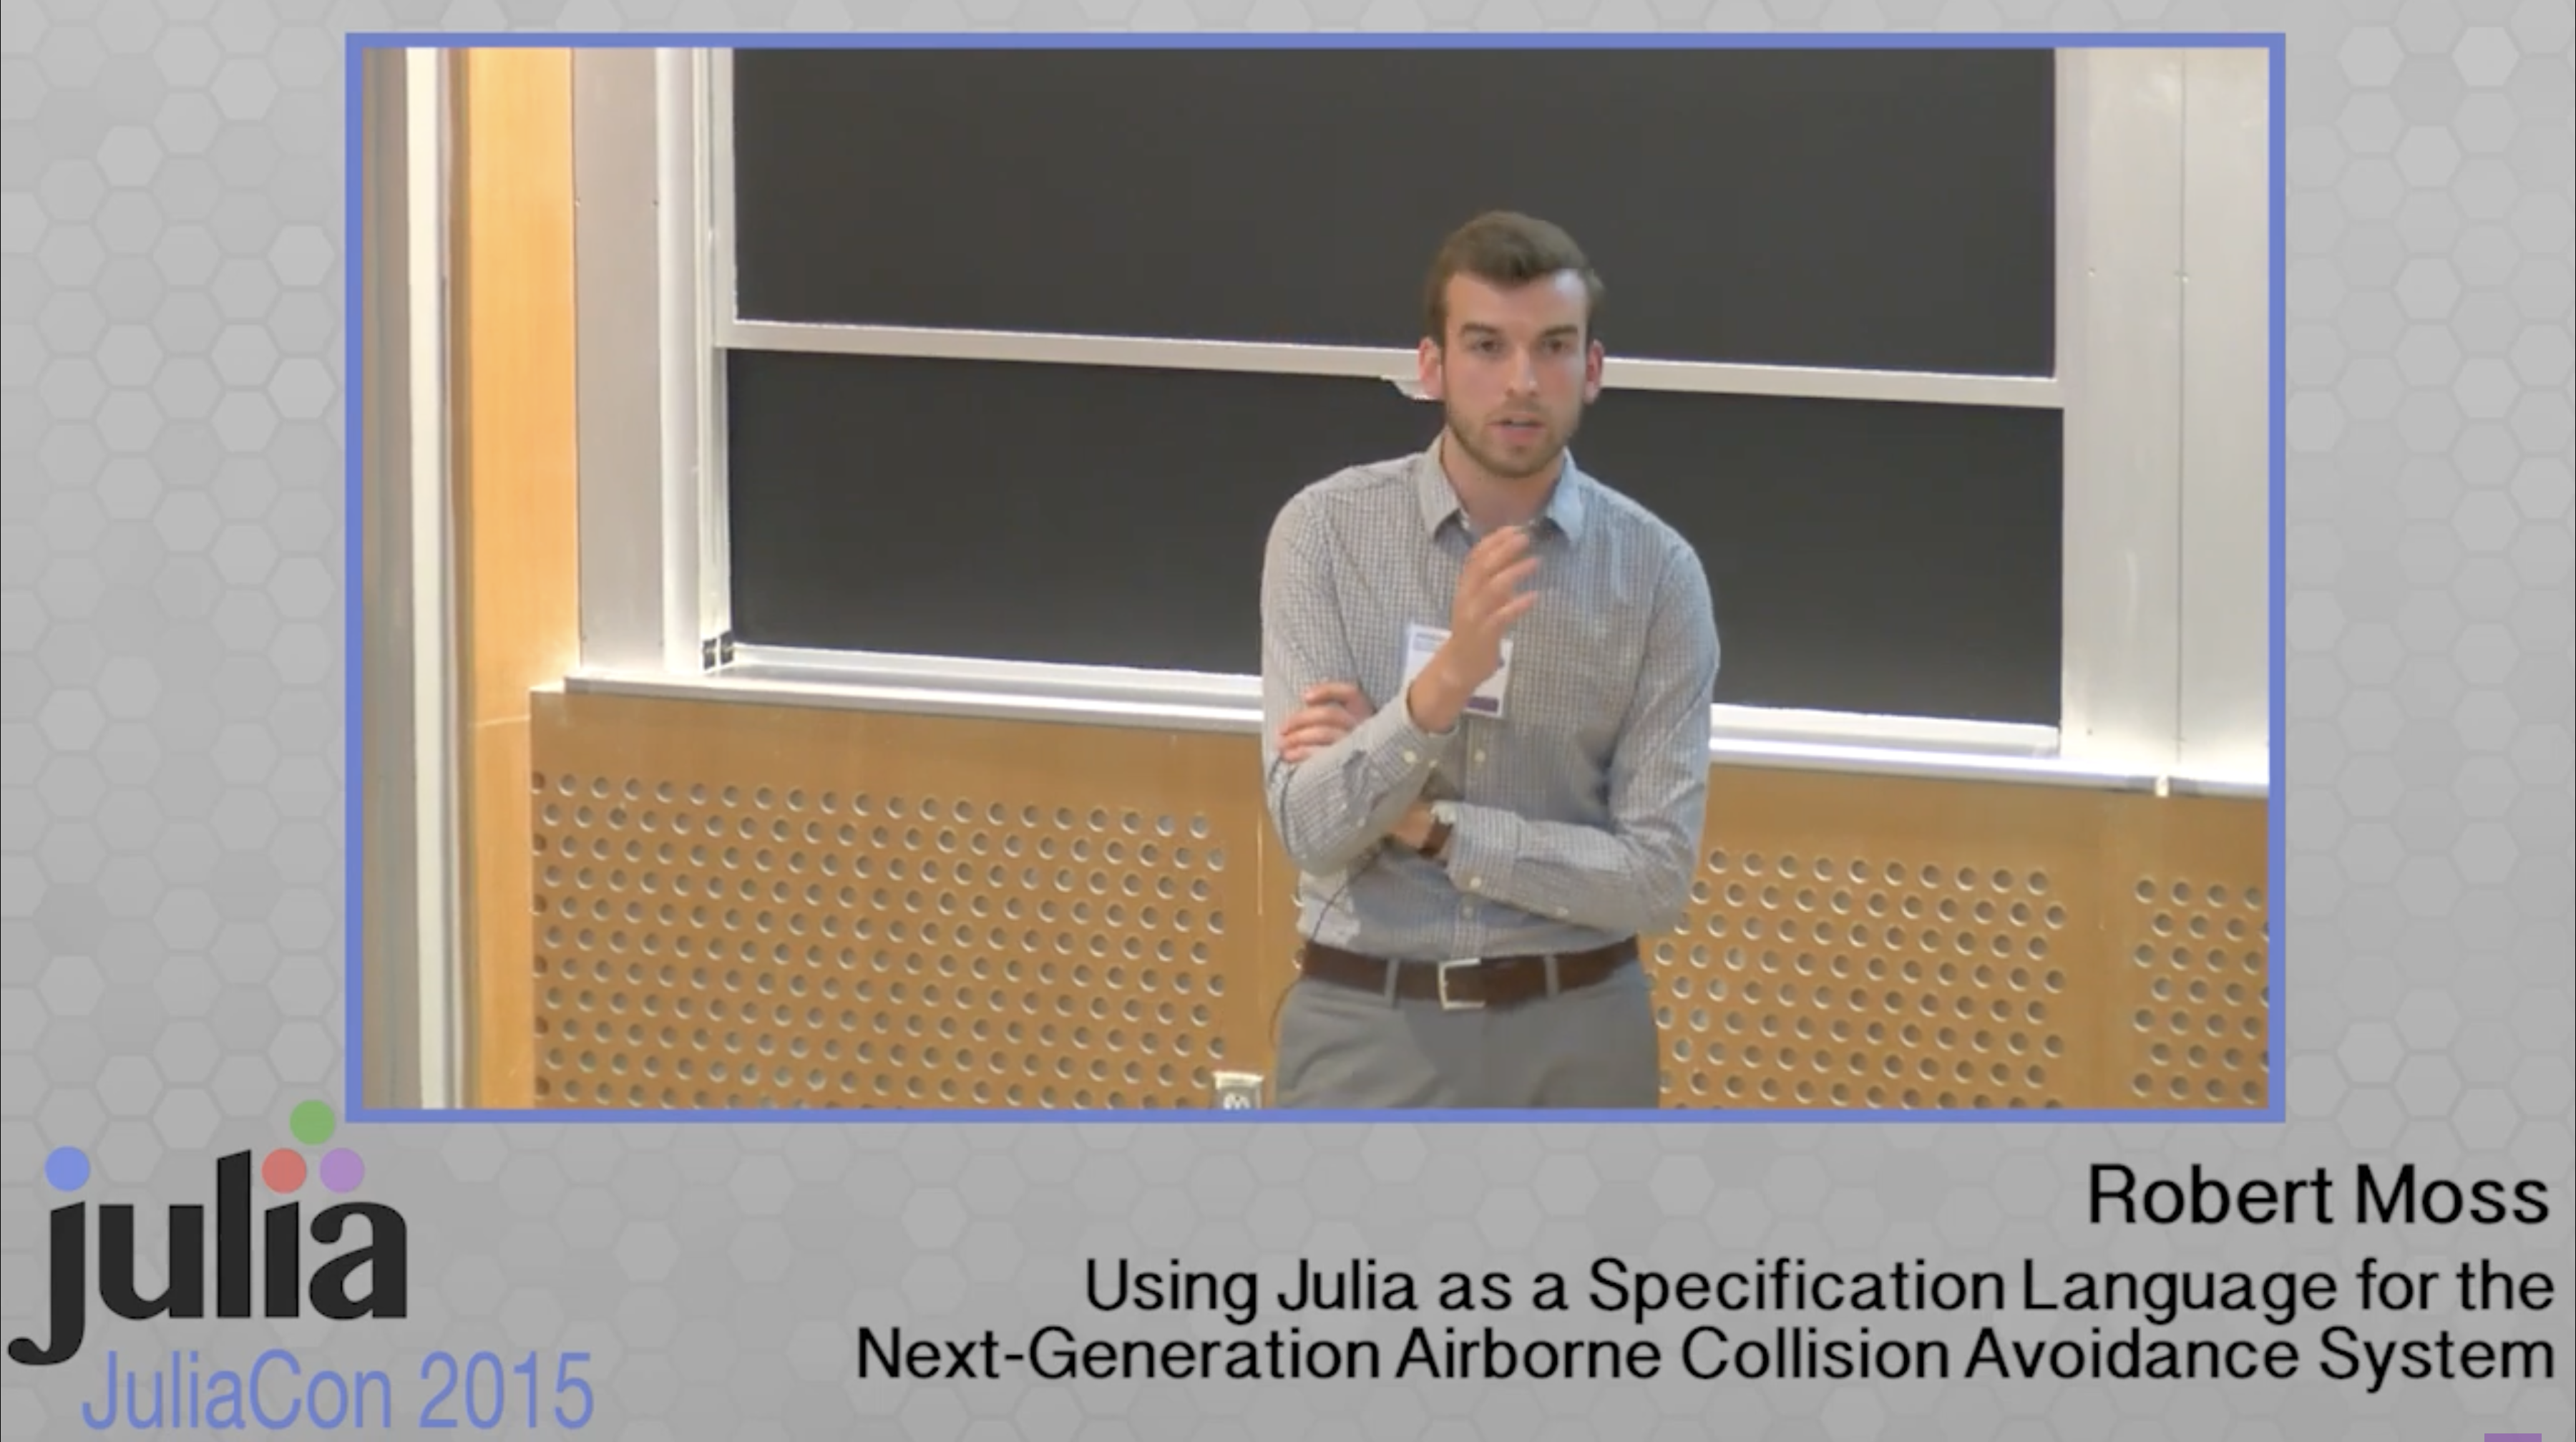
\includegraphics[width=\linewidth]{media/juliacon-2015.png}
        };
    \end{tikzpicture}

    \captionof*{figure}{\shortstack{\footnotesize Prev. at MIT Lincoln Laboratory\\\textcolor{gray}{\scriptsize Julia as a specification language}}}
  \end{column}

  \pause

  \begin{column}{0.33\textwidth}
    \centering
    
\includegraphics[width=\linewidth]{media/textbook-cover.png}
    
    \captionof*{figure}{\shortstack{\footnotesize Textbook Co-Author/Head TA\\\textcolor{gray}{\scriptsize Algorithms written in Julia}}}
  \end{column}

\end{columns}

\end{frame}
\begin{frame}[fragile]{Textbooks using Julia}
    
\pause

\begin{columns}

  \begin{column}{0.30\textwidth}
    \centering
    \begin{tikzpicture}
        \node[draw=white, line width=1pt, inner sep=0pt] {
            
\includegraphics[width=\linewidth]{media/algforopt.png}
        };
    \end{tikzpicture}
    
    \captionof*{figure}{\shortstack{\footnotesize Algorithms for Optimization\\\textcolor{gray}{\scriptsize MIT Press, 2019}}}
  \end{column}

  \pause

  \begin{column}{0.30\textwidth}
    \centering
    \begin{tikzpicture}
        \node[draw=white, line width=1pt, inner sep=0pt] {
            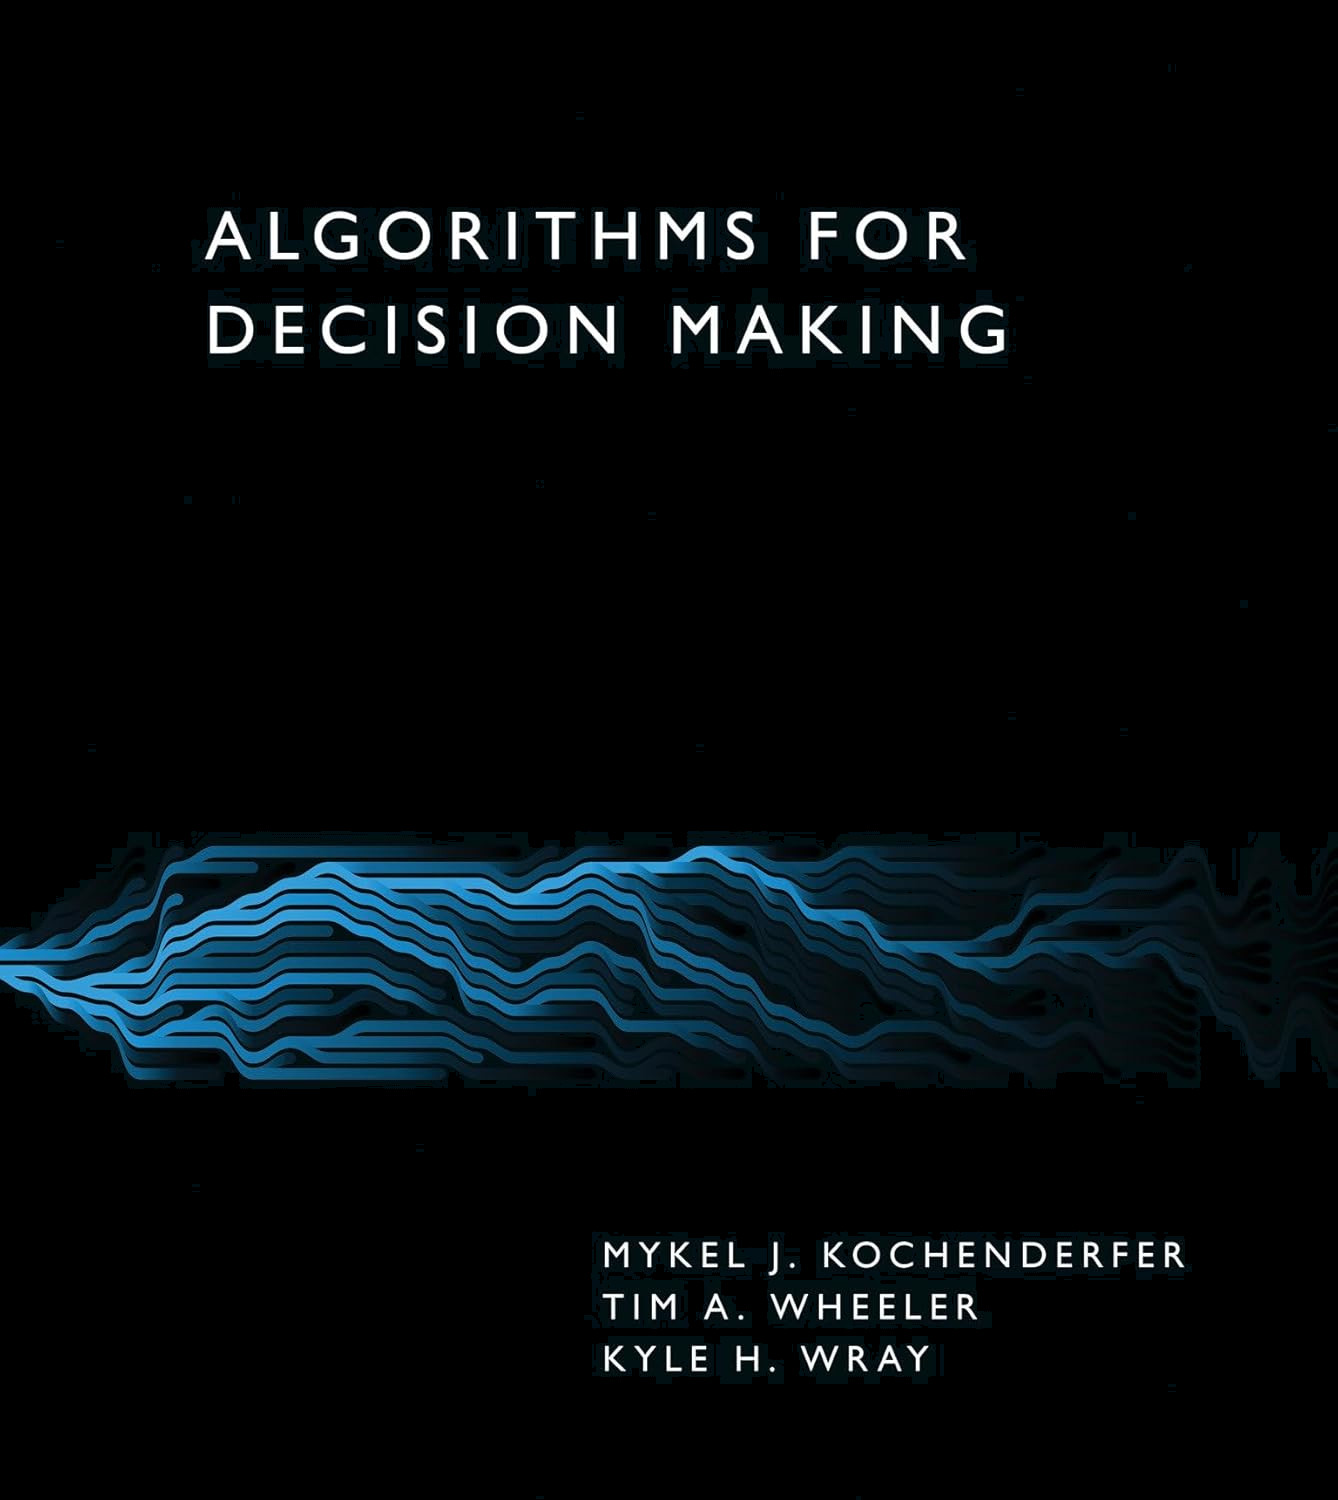
\includegraphics[width=\linewidth]{media/algfordm.png}
        };
    \end{tikzpicture}

    \captionof*{figure}{\shortstack{\footnotesize Algorithms for Decision Making\\\textcolor{gray}{\scriptsize MIT Press, 2022}}}
  \end{column}

  \pause

  \begin{column}{0.30\textwidth}
    \centering
    \begin{tikzpicture}
        \node[draw=white, line width=1pt, inner sep=0pt] {
            
\includegraphics[width=\linewidth]{media/algforval.png}
        };
    \end{tikzpicture}

    \captionof*{figure}{\shortstack{\footnotesize Algorithms for Validation\\\textcolor{gray}{\scriptsize MIT Press, 2025}}}
  \end{column}

\end{columns}

\pause

\small
\centering
All PDFs available for free at \textcolor{repo}{\texttt{https://algorithmsbook.com}}

\end{frame}
\begin{frame}[fragile]{\shortstack[l]{JuliaCon 2019}}

\centering

\includegraphics[width=0.7\linewidth]{media/textbook-juliacon-2019.png}

\phantom{---}

\shortstack{\footnotesize How We Wrote a Textbook using Julia\\\textcolor{gray}{\scriptsize Tim Wheeler, JuliaCon 2019}}

\end{frame}
\begin{frame}[fragile]{Textbooks with integrated Julia}
    
\pause

\begin{columns}

  \begin{column}{0.30\textwidth}
    \centering
    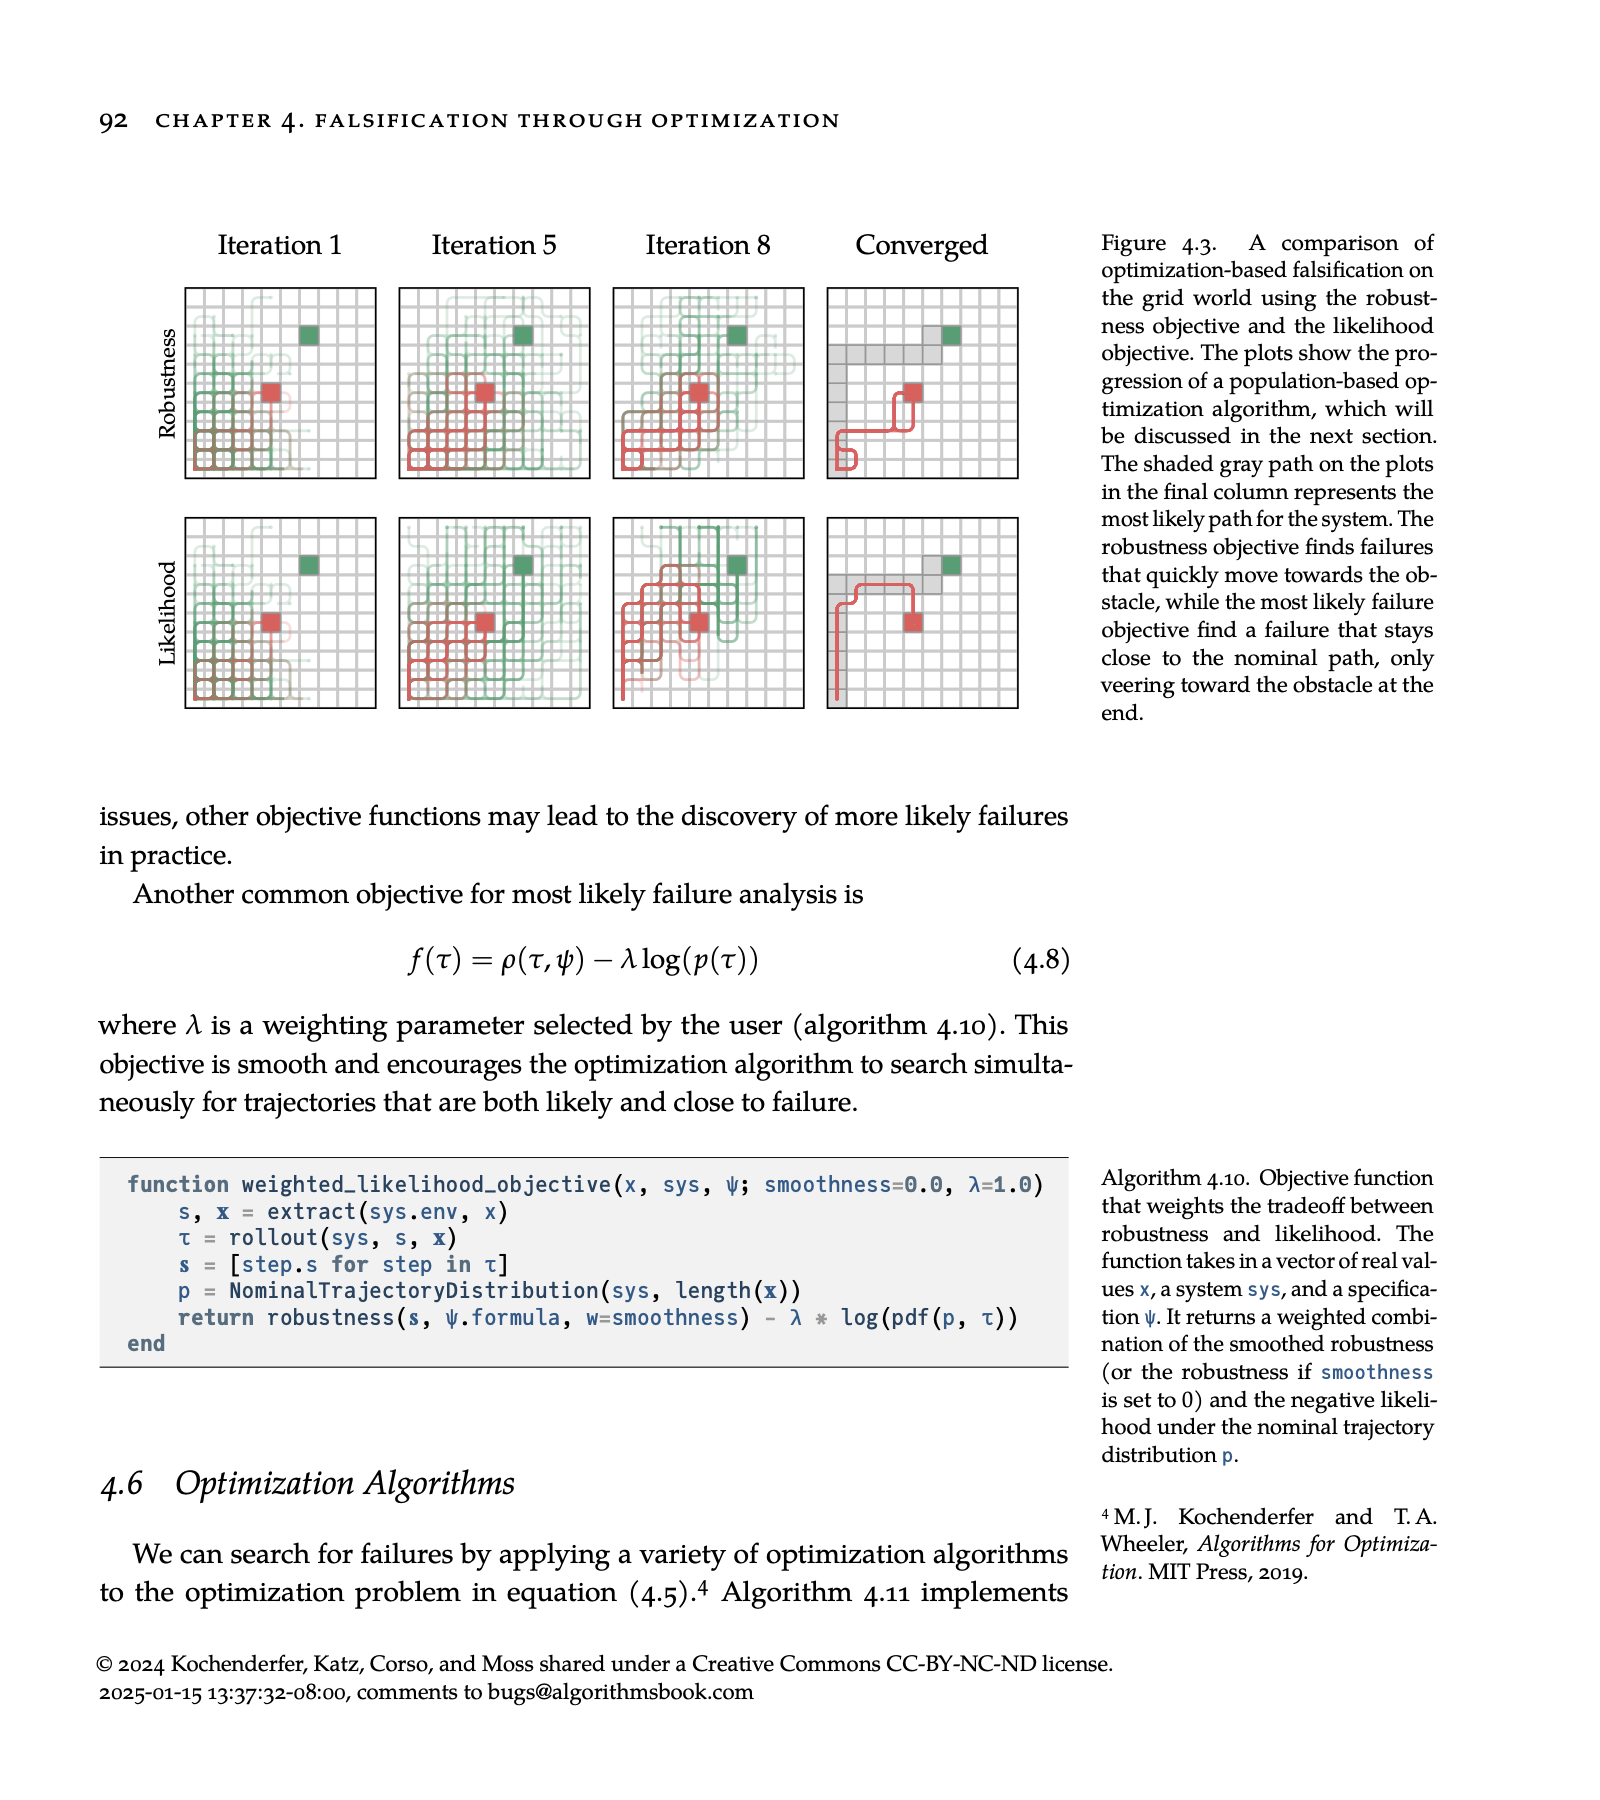
\includegraphics[width=\linewidth]{media/val-pg92.png}
    
    \captionof*{figure}{\shortstack{\footnotesize Algorithms for Validation\\\textcolor{gray}{\scriptsize Figures and Julia code}}}
  \end{column}

  \pause

  \begin{column}{0.66\textwidth}
    % \begin{itemize}
    %   \item Written in Julia
    % \end{itemize}
    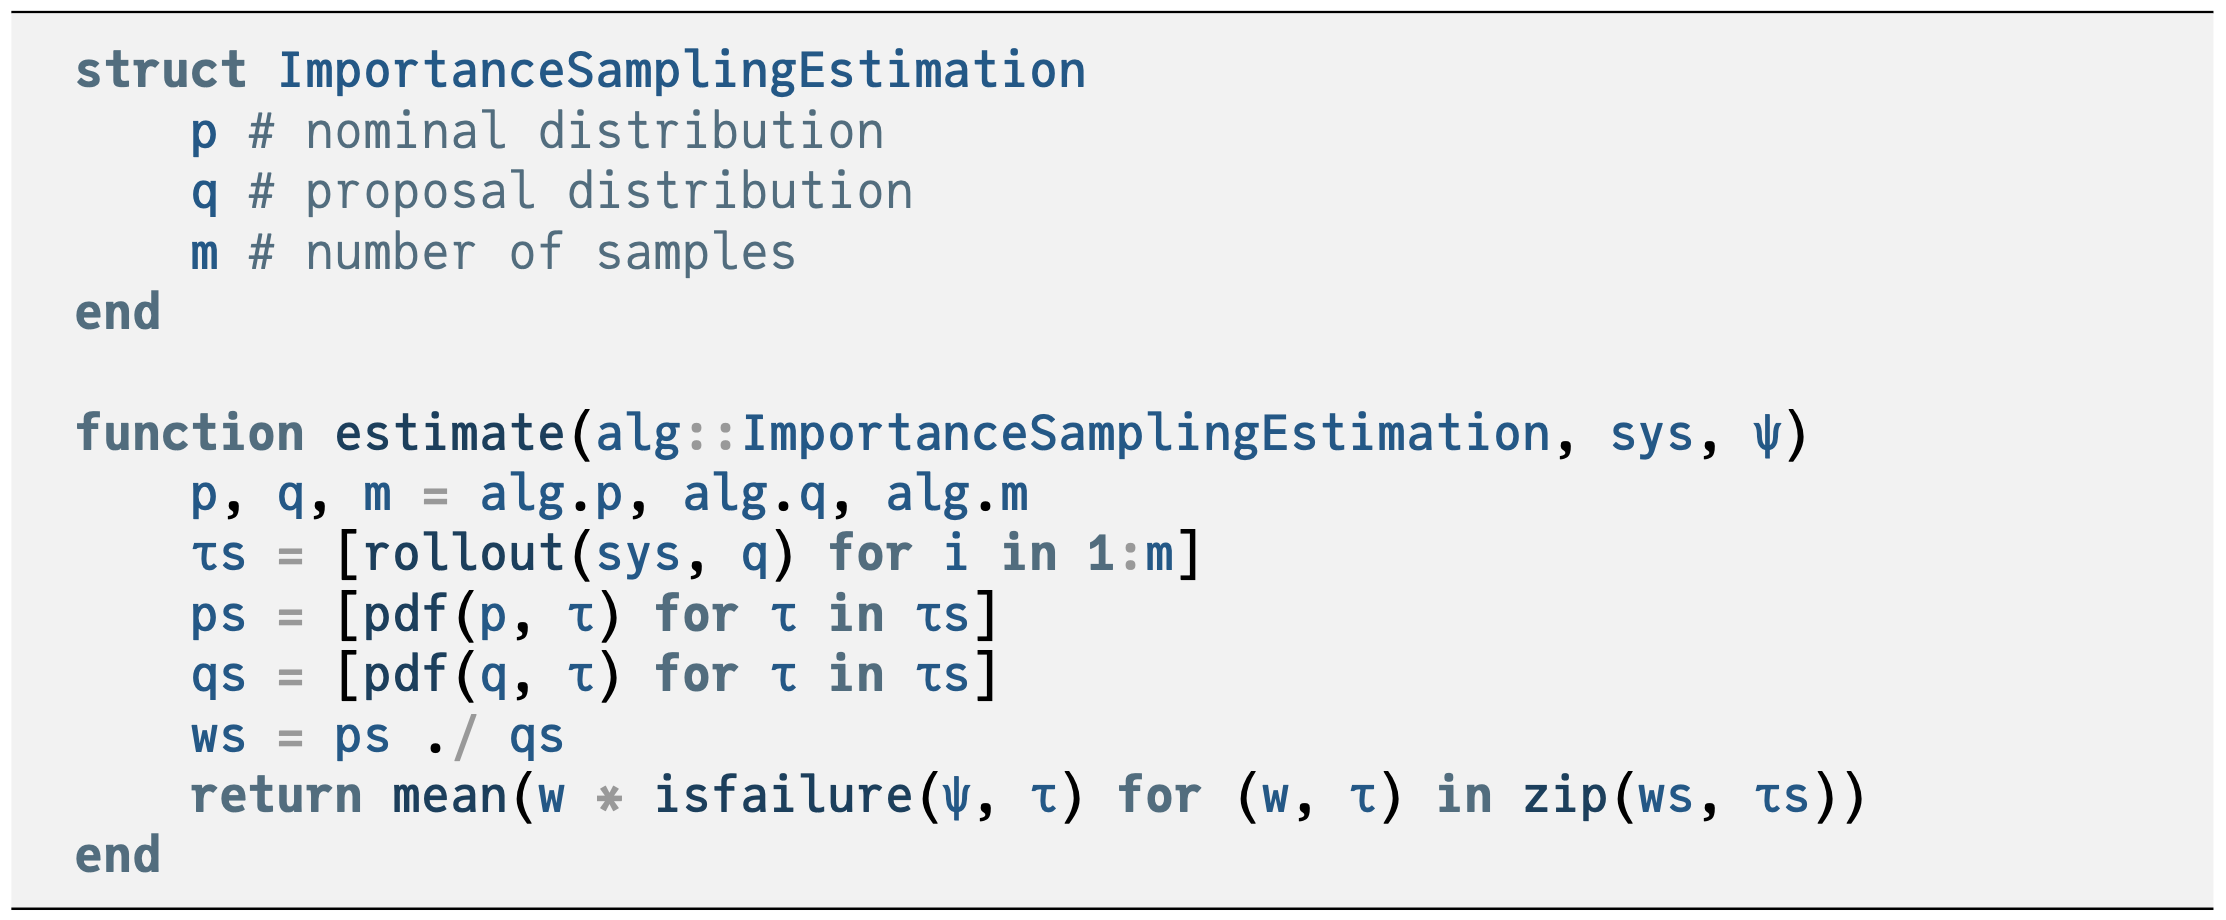
\includegraphics[width=\linewidth]{media/is.png}
    
    \captionof*{figure}{\shortstack{\footnotesize Example algorithm\\\textcolor{gray}{\scriptsize Importance sampling estimation of failure probability}}}
  \end{column}

\end{columns}

\end{frame}
\begin{frame}[fragile]{Julia integrated into \LaTeX{} code}

\begin{columns}
  \hfill
  \begin{column}{0.33\textwidth}
    \begin{minipage}[t]{\linewidth}
      \centering
      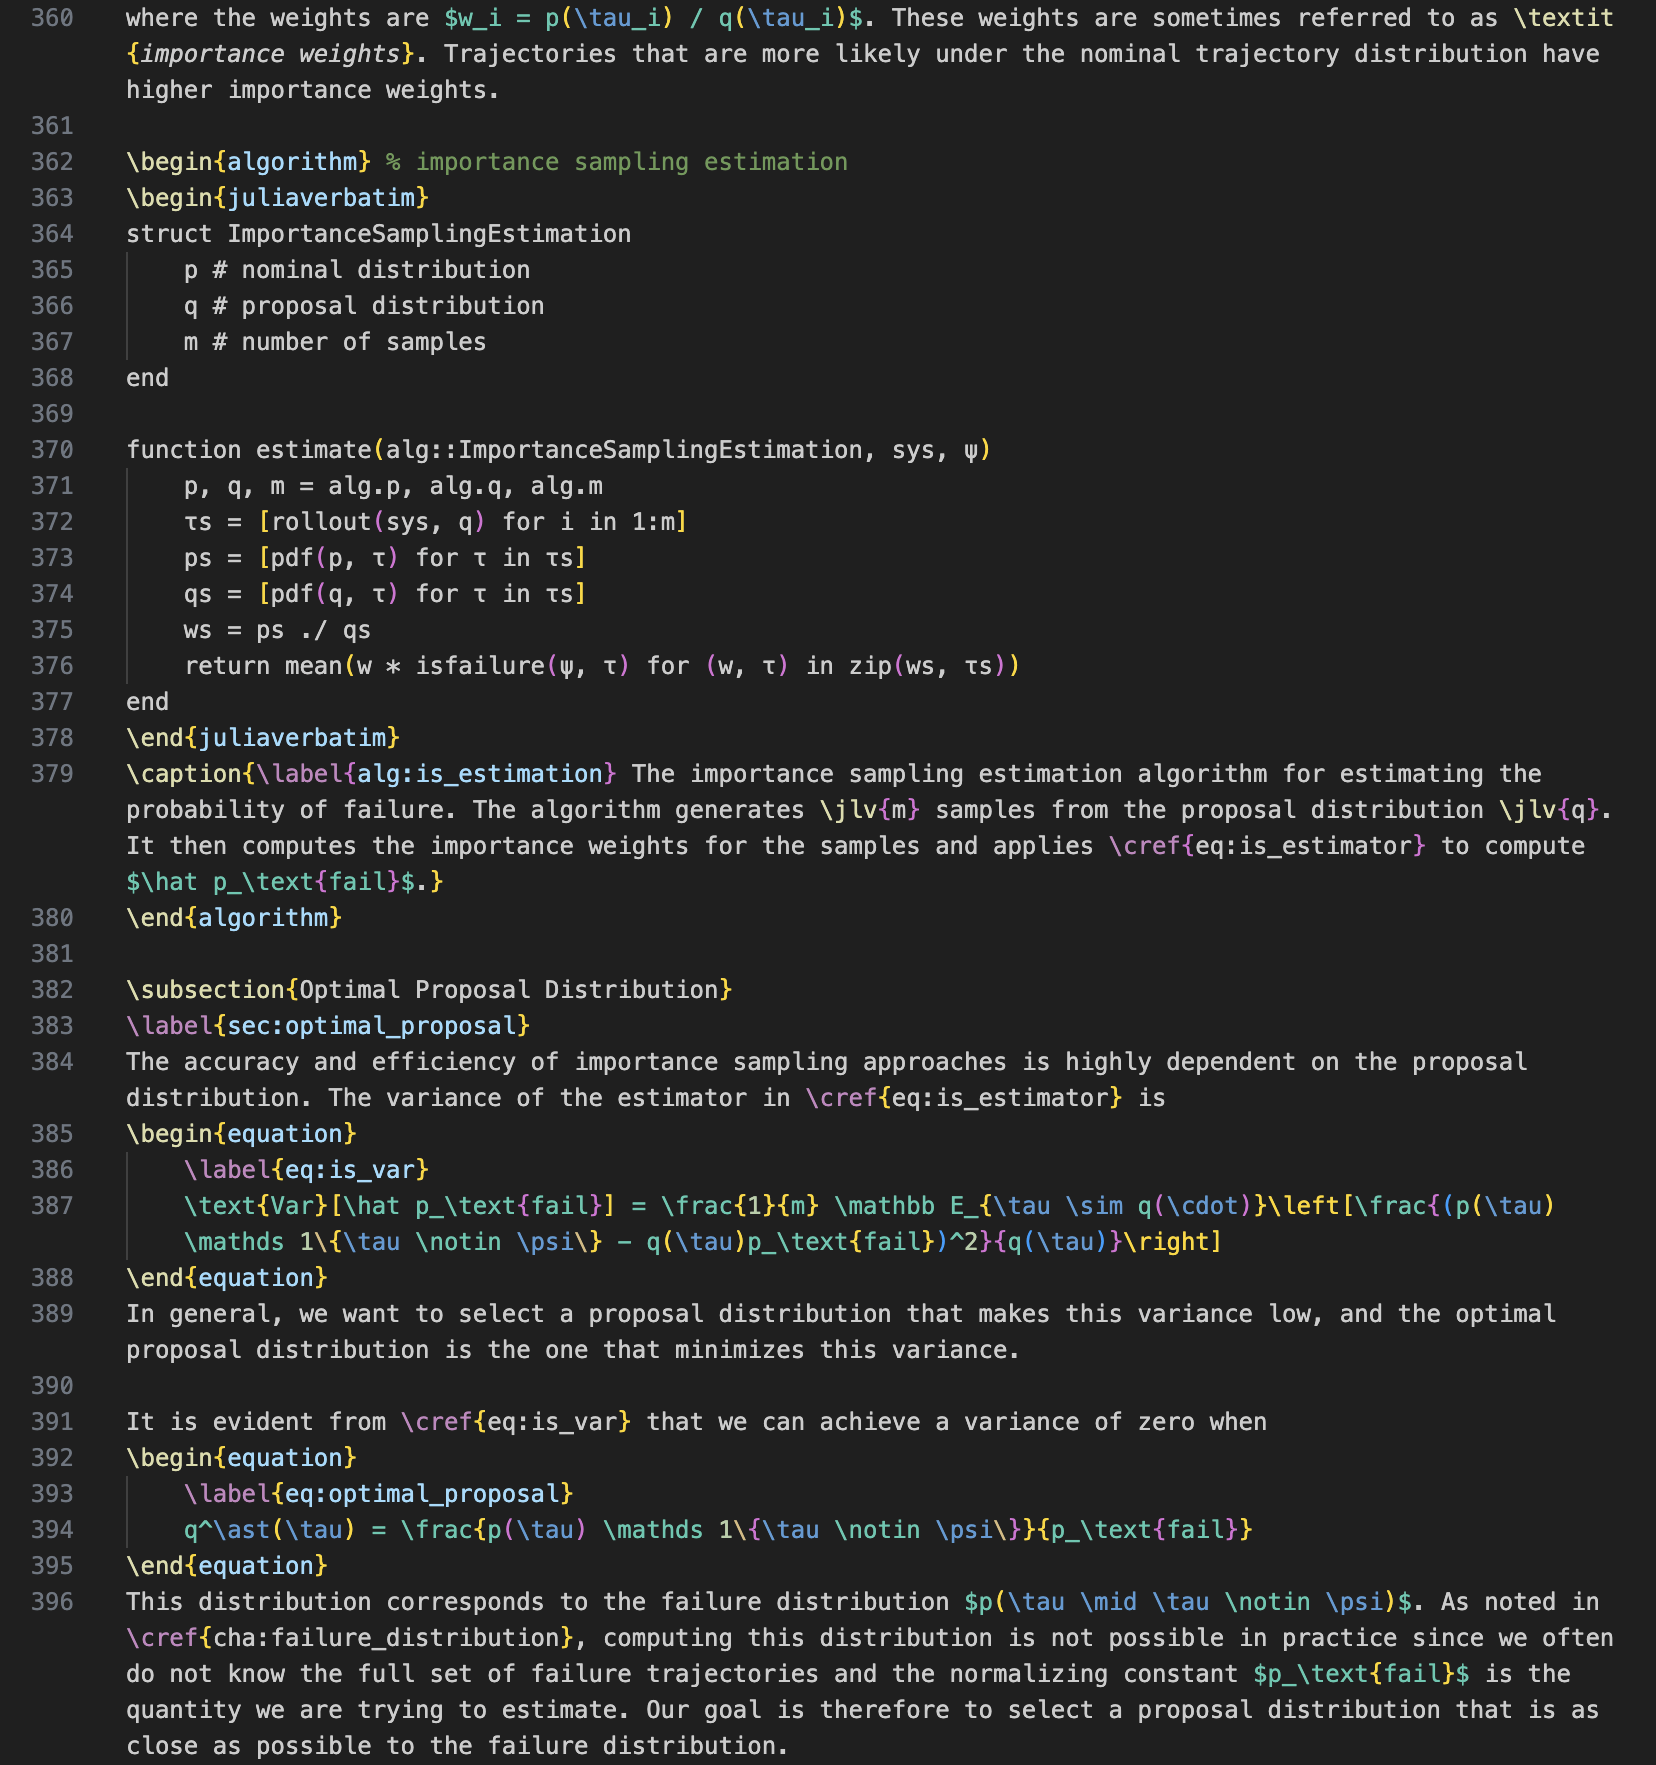
\includegraphics[width=\linewidth]{media/val-pg147-latex.png}

      \captionof*{figure}{\shortstack{\footnotesize \LaTeX{} code example\\\textcolor{gray}{\scriptsize Integrated Julia code using \jlv{pythontex}}}}
    \end{minipage}
  \end{column}
  \pause
  \begin{column}{0.33\textwidth}
    \centering
    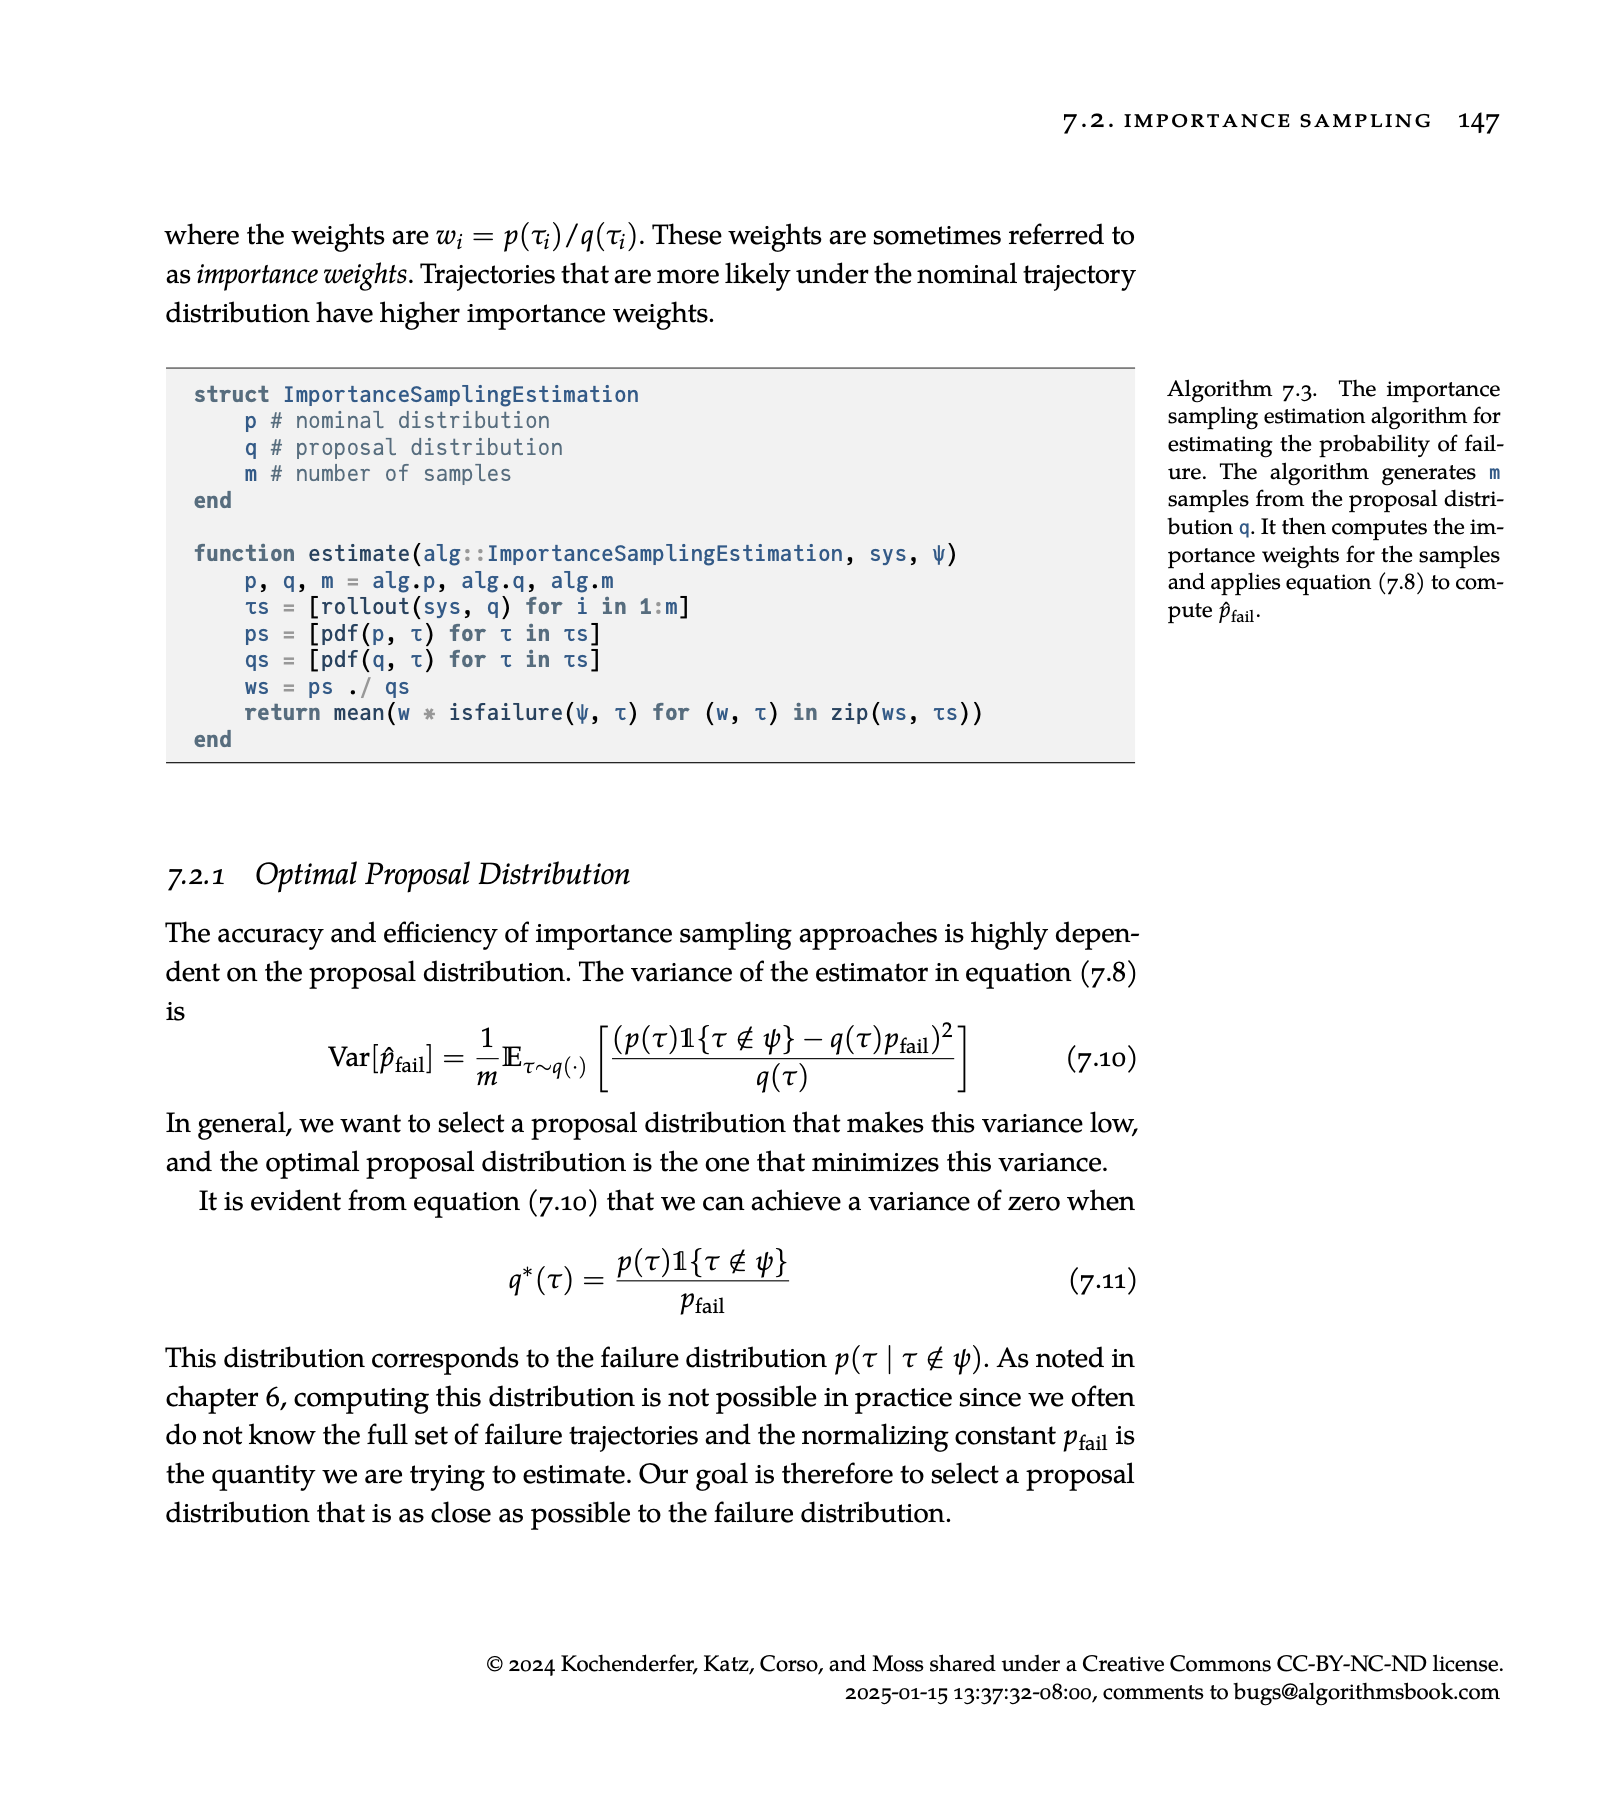
\includegraphics[width=\linewidth]{media/val-pg147.png}
    
    \captionof*{figure}{\shortstack{\footnotesize Compiled \LaTeX{} PDF\\\textcolor{gray}{\scriptsize Julia algorithms and \LaTeX{} math}}}
  \end{column}
  \hfill
\end{columns}

\end{frame}
\begin{frame}[fragile]{Open-Source Textbook Template Repository} \pause

\centering

\includegraphics[width=0.5\linewidth]{media/tufte_algorithms_book.png}

\textcolor{repo}{\small \texttt{github.com/sisl/tufte\_algorithms\_book}}

\end{frame}
\begin{frame}[fragile]{Open-Source Slides Repo (\jlv{beamer} + \jlv{pythontex})} \pause

\centering


\includegraphics[width=0.5\linewidth]{media/julia-in-academia.png}

\textcolor{repo}{\small \texttt{github.com/mossr/julia-in-academia}}

\pause

\phantom{---}

\phantom{---}


\includegraphics[width=0.5\linewidth]{media/julia-tufte-beamer.png}

\textcolor{repo}{\small \texttt{github.com/mossr/julia-tufte-beamer}}

\end{frame}
\begin{frame}[fragile,t]{Integrated Julia Example}

\phantom{}

We can compute Julia code \textit{directly in the slides/pages}.
% You can also compute the \textit{robustness} of a trajectory $\tau$.

\phantom{}

\begin{footnotesize}
\begin{juliaconsole}
using SignalTemporalLogic
τ = [-1.0, -3.2, 2.0, 1.5, 3.0, 0.5, -0.5, -2.0, -4.0, -1.5];
ψ₁ = @formula ◊(sₜ -> sₜ > 0);
ρ₁ = ρ(τ, ψ₁)
ψ₂ = @formula □(sₜ -> sₜ > 0);
ρ₂ = ρ(τ, ψ₂)
\end{juliaconsole}
\onslide<1>{\lineblackout{7}}
\onslide<1-2>{\lineblackout{6}\lineblackout{5}}
\onslide<1-3>{\lineblackout{4}\lineblackout{3}}
\onslide<1-4>{\lineblackout{2}}
\onslide<1-5>{\lineblackout{1}\lineblackout{0}}
\onslide<6>{}
\end{footnotesize}

\vspace*{5pt}

\pause\pause
{\footnotesize\jlv{τ  # \tau<TAB>}}

{\footnotesize\jlv{ψ₁ # \psi<TAB>\_1<TAB>}}

{\footnotesize\jlv{◊  # \lozenge<TAB>}}

\pause
{\footnotesize\jlv{ρ  # \rho<TAB>}}

\pause
{\footnotesize\jlv{□  # \square<TAB>}}

\begin{figure}
    \begin{jlcode}
    p = let
        times = collect(1:10)
        τ = [-1.0, -3.2, 2.0, 1.5, 3.0, 0.5, -0.5, -2.0, -4.0, -1.5];

        xmin, xmax, ymin, ymax = 1, 10, -5, 4
        ax = Axis(xmin=xmin, xmax=xmax, ymin=ymin, ymax=ymax, width="9cm", height="4.5cm")
        ax.xlabel = "Time"
        ax.ylabel = L"s"
        ax.title = raw"${\color{pastelSkyBlue}\psi_1 = \lozenge\big( s_t > 0 \big)} \qquad {\color{pastelGreen}\psi_2 = \square\big( s_t > 0 \big)}$"
        ax.style = raw"title style={font=\footnotesize}"

        # Used to add phantom right yaxis for better centering
        axr = deepcopy(ax)
        axr.style *= raw", axis y line*=right, axis x line=none, yticklabel={\phantom{\pgfmathprintnumber{\tick}}}"
        axr.ylabel = "\\phantom{$(ax.ylabel)}"
        push!(axr, Plots.Command(""))

        push!(ax, Plots.Linear(times, τ, style="solid, mark=*, gray, line width=1pt, mark options={fill=gray!50, draw=gray}, mark size=2pt"))
        push!(ax, Plots.Linear([xmin, xmax], [0, 0], style="dotted, mark=none, gray, line width=1pt"))
        push!(ax, Plots.Scatter([5], [3], style="only marks, mark=*, mark size=2pt, mark options={fill=pastelSkyBlue!50, draw=pastelSkyBlue}"))
        push!(ax, Plots.Linear([xmin, xmax], [3, 3], style="dashed, mark=none, pastelSkyBlue, line width=1pt"))
        push!(ax, Plots.Command("\\node[anchor=center] at (axis cs: 8, 2.3) {\\scriptsize \\textcolor{pastelSkyBlue}{\$\\rho_1\$}};"))
        push!(ax, Plots.Scatter([9], [-4], style="only marks, mark=*, mark size=2pt, mark options={fill=pastelGreen!50, draw=pastelGreen}"))
        push!(ax, Plots.Linear([xmin, xmax], [-4, -4], style="dashed, mark=none, pastelGreen, line width=1pt"))
        push!(ax, Plots.Command("\\node[anchor=center] at (axis cs: 5, -3.3) {\\scriptsize \\textcolor{pastelGreen}{\$\\rho_2\$}};"))
        [axr, ax]
    end
    plot(p)
    \end{jlcode}
\end{figure}

\onslide<7>{\begin{tikzpicture}[remember picture, overlay]
    \node[anchor=south east] at ($(current page.south east)+(0.4cm,0.15cm)$) {
        \input{fig/jl_robustness}
    };
\end{tikzpicture}}

\end{frame}

\begin{frame}[fragile]{Julia for Textbooks: \textcolor{paloalto}{The Good}} \pause

\begin{itemize}
  \item \textcolor{paloalto}{Concise} algorithm descriptions (fits within single page) \pause
  \item \textcolor{paloalto}{Multiple dispatch} makes it easy to design common interface \pause
  \item \textcolor{paloalto}{Auto-differentiation} allows for clean algorithms that just work \pause
  \item \textcolor{paloalto}{Full Unicode support} means math matches code (e.g., $\lambda$ in math and \jlv{λ} in code)
\end{itemize}

\pause

\phantom{---}

\small
\shortstack[l]{\textbf{Shout-out to the following packages}:\\\jlv{Distributions.jl}, \jlv{LazySets.jl}, \jlv{IntervalArithmetic.jl}, \jlv{Flux.jl}, \jlv{Optim.jl}, and \jlv{JuMP.jl}}

\end{frame}
\begin{frame}[fragile]{Showcase: \normalfont\jlv{IntervalArithmetic.jl} and \jlv{LazySets.jl}} \pause

{\scriptsize
\begin{algorithmblock}
\begin{juliaverbatim}
struct NaturalInclusion <: ReachabilityAlgorithm
    h # time horizon
end

function r(sys, x)
    s, 𝐱 = extract(sys.env, x)
    τ = rollout(sys, s, 𝐱)
    return τ[end].s
end

to_hyperrectangle(𝐈) = Hyperrectangle(low=[i.lo for i in 𝐈], 
                                      high=[i.hi for i in 𝐈])

function reachable(alg::NaturalInclusion, sys)
    𝐈′s = []
    for d in 1:alg.h
        𝐈 = intervals(sys, d)
        push!(𝐈′s, r(sys, 𝐈))
    end
    return UnionSetArray([to_hyperrectangle(𝐈′) for 𝐈′ in 𝐈′s])
end
\end{juliaverbatim}
\end{algorithmblock}
}

\end{frame}


\begin{frame}[fragile]{Showcase: \normalfont\jlv{IntervalArithmetic.jl} and \jlv{LazySets.jl}}

\begin{figure} % interval counterparts
    \begin{jlcode}
    p = let
        xmin, xmax, ymin, ymax = 0, 2.75, 0, 10
        ax1 = plot_interval(exp, interval(1, 2), interval(exp(1), exp(2)), xmin, xmax, ymin, ymax, fxmax=log(ymax), color="pastelSkyBlue")
        ax1.xlabel = L"x"
        ax1.ylabel = L"f(x)"
        ax1.title = L"f(x) = \exp(x)"
        ax1.height = "4.5cm"
        ax1.width = "4.5cm"

        xmin, xmax, ymin, ymax = -2, 2, 0, 4.5
        ax2 = plot_interval(x->x^2, interval(-1.5, 1), interval(0, 1.5^2), xmin, xmax, ymin, ymax, color="pastelSkyBlue")
        ax2.xlabel = L"x"
        ax2.title = L"\phantom{\sin(x)}f(x) = x^2\phantom{\sin(x)}"
        ax2.height = "4.5cm"
        ax2.width = "4.5cm"

        xmin, xmax, ymin, ymax = -3.14, 3.14, -1.5, 1.5
        ax3 = plot_interval(sin, interval(0, 2), interval(0, 1), xmin, xmax, ymin, ymax, color="pastelSkyBlue")
        ax3.xlabel = L"x"
        ax3.title = L"f(x) = \sin(x)"
        ax3.height = "4.5cm"
        ax3.width = "4.5cm"

        g = GroupPlot(3, 1, groupStyle="horizontal sep=1cm")
        push!(g, ax1)
        push!(g, ax2)
        push!(g, ax3)
        g
    end
    plot(p)
    \end{jlcode}
    \begin{center}
        \plot{fig/interval_counterparts}
    \end{center}
	\caption{Example of the interval counterparts for the $\exp$, square, and $\sin$ functions.}
\end{figure}

\end{frame}


\begin{frame}[fragile]{Showcase: \normalfont\jlv{IntervalArithmetic.jl} and \jlv{LazySets.jl}}

{\small
\begin{algorithmblock}
\begin{juliaverbatim}
function (env::InvertedPendulum)(s, a)
    θ, ω = s[1], s[2]
    dt, g, m, l = env.dt, env.g, env.m, env.l
    ω = ω + (3g / (2 * l) * sin(θ) + 3 * a / (m * l^2)) * dt
    θ = θ + ω * dt
    return [θ, ω]
end
\end{juliaverbatim}
\end{algorithmblock}
}

\end{frame}


\begin{frame}[fragile]{Showcase: \normalfont\jlv{IntervalArithmetic.jl} and \jlv{LazySets.jl}}
    
\begin{figure}
    \begin{jlcode}
    function intervals(sys, d)
        disturbance_mag = 0.01
        θmin, θmax = -π/16, π/16
        ωmin, ωmax =  -1.0, 1.0
        𝐈 = [interval(θmin, θmax), interval(ωmin, ωmax)]
        for i in 1:d
            push!(𝐈, interval(-disturbance_mag, disturbance_mag))
            push!(𝐈, interval(-disturbance_mag, disturbance_mag))
        end
        return 𝐈
    end
    function extract(env::InvertedPendulum, x)
        s = x[1:2]
        𝐱 = [Disturbance(0, 0, x[i:i+1]) for i in 3:2:length(x)]
        return s, 𝐱
    end
    p = let
        agent = ProportionalController([-15., -8.])
        env = InvertedPendulum()
        disturbance_mag = 0.01
        θmin, θmax = -π/16, π/16
        ωmin, ωmax =  -1.0, 1.0
        sensor = AdditiveNoiseSensor(Product([Uniform(-disturbance_mag, disturbance_mag), Uniform(-disturbance_mag, disturbance_mag)]))
        Ps(env::InvertedPendulum) = Product([Uniform(θmin, θmax), Uniform(ωmin, ωmax)])
        inverted_pendulum = System(agent, env, sensor)

        d = 2
        Random.seed!(4)
        τs = [rollout(inverted_pendulum, d=d) for i in 1:150]
        sfinals = [τ[end].s for τ in τs]

        alg = NaturalInclusion(d)
        ℛ = reachable(alg, inverted_pendulum)

        ax = inv_pendulum_state_space(ymin=-3, ymax=3)
        push!(ax, Plots.Scatter([s[1] for s in sfinals], [s[2] for s in sfinals], 
            style="solid, mark=*, mark size=1pt, mark options={draw=pastelSkyBlue, fill=pastelSkyBlue!80, fill opacity=1.0, draw opacity=1.0}"))
        plot_polytope!(ax, ℛ[2], fill_color="pastelPurple!20!black", draw_color="pastelPurple", fill_alpha=1.0, draw_alpha=1.0)
        ax.height = "4.5cm"
        ax.width = "4.5cm"
        ax
    end
    plot(p)
    \end{jlcode}
    \begin{center}
        \plot{fig/natural_inclusion_pendulum}
    \end{center}
    \caption{Reachable set for the inverted pendulum system.}
\end{figure}

\end{frame}

\begin{frame}[fragile]{\textbf{Julia for Textbooks}: \textcolor{cardinal}{The Not-So-Good}}
    
\pause

\begin{itemize}
  \item \textcolor{cardinal}{Somewhat new to readers:} Requires learning Julia in the process \pause
  \item \textcolor{cardinal}{Potential obscure idioms:} broadcasting, anonymous functions, multiple dispatch \pause
  \item \textcolor{cardinal}{Textbook tooling:} Needed to be built out from scratch
\end{itemize}

\end{frame}
\begin{frame}[fragile]{Julia in the Classroom} \pause

\centering

\includegraphics[width=0.5\linewidth]{media/aa228v.png}

{\footnotesize Grad-level course at Stanford}

\textcolor{gray}{\scriptsize Follows \textit{Algorithms for Validation} textbook}

\textcolor{gray}{\scriptsize First offered in Winter 2025}

\end{frame}
\begin{frame}[fragile]{Lectures} \pause

\centering
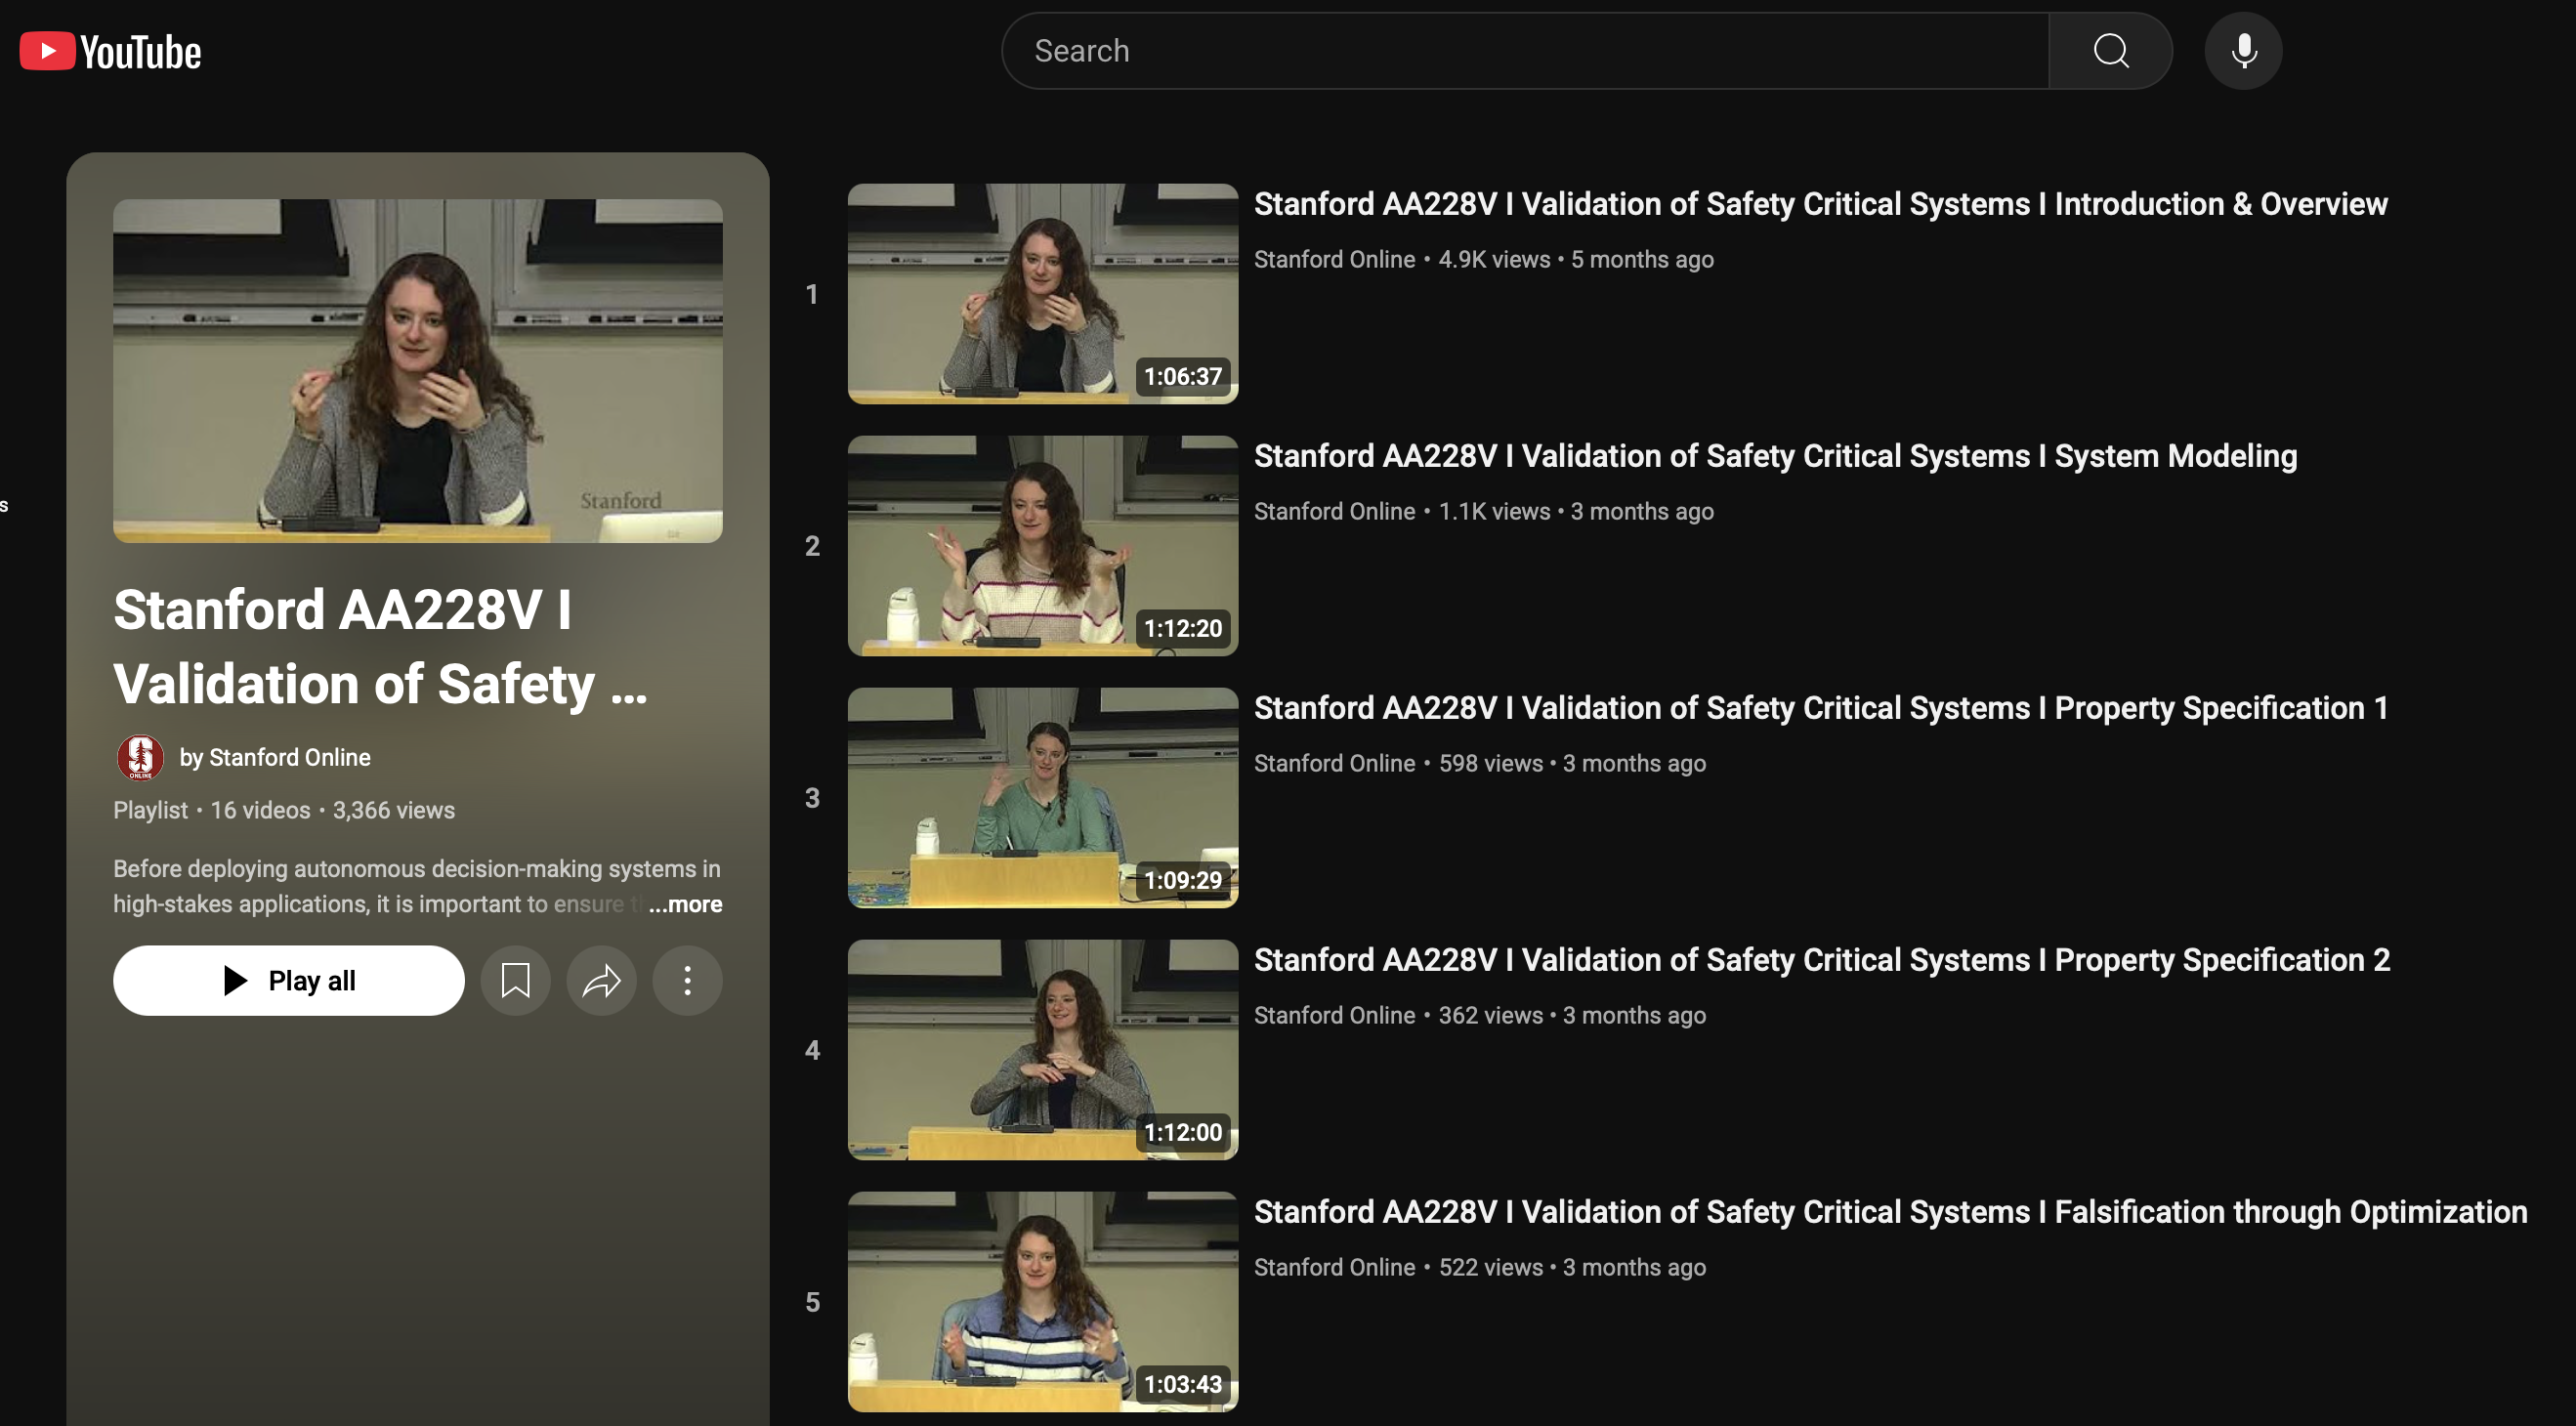
\includegraphics[width=0.7\linewidth]{media/aa228v-lectures.png}

{\footnotesize All lectures available on YouTube}

\textcolor{gray}{\scriptsize Led by Sydney Katz, textbook co-author and award-winning lecturer}

\end{frame}
\begin{frame}[fragile]{Interactive Lectures}

\centering
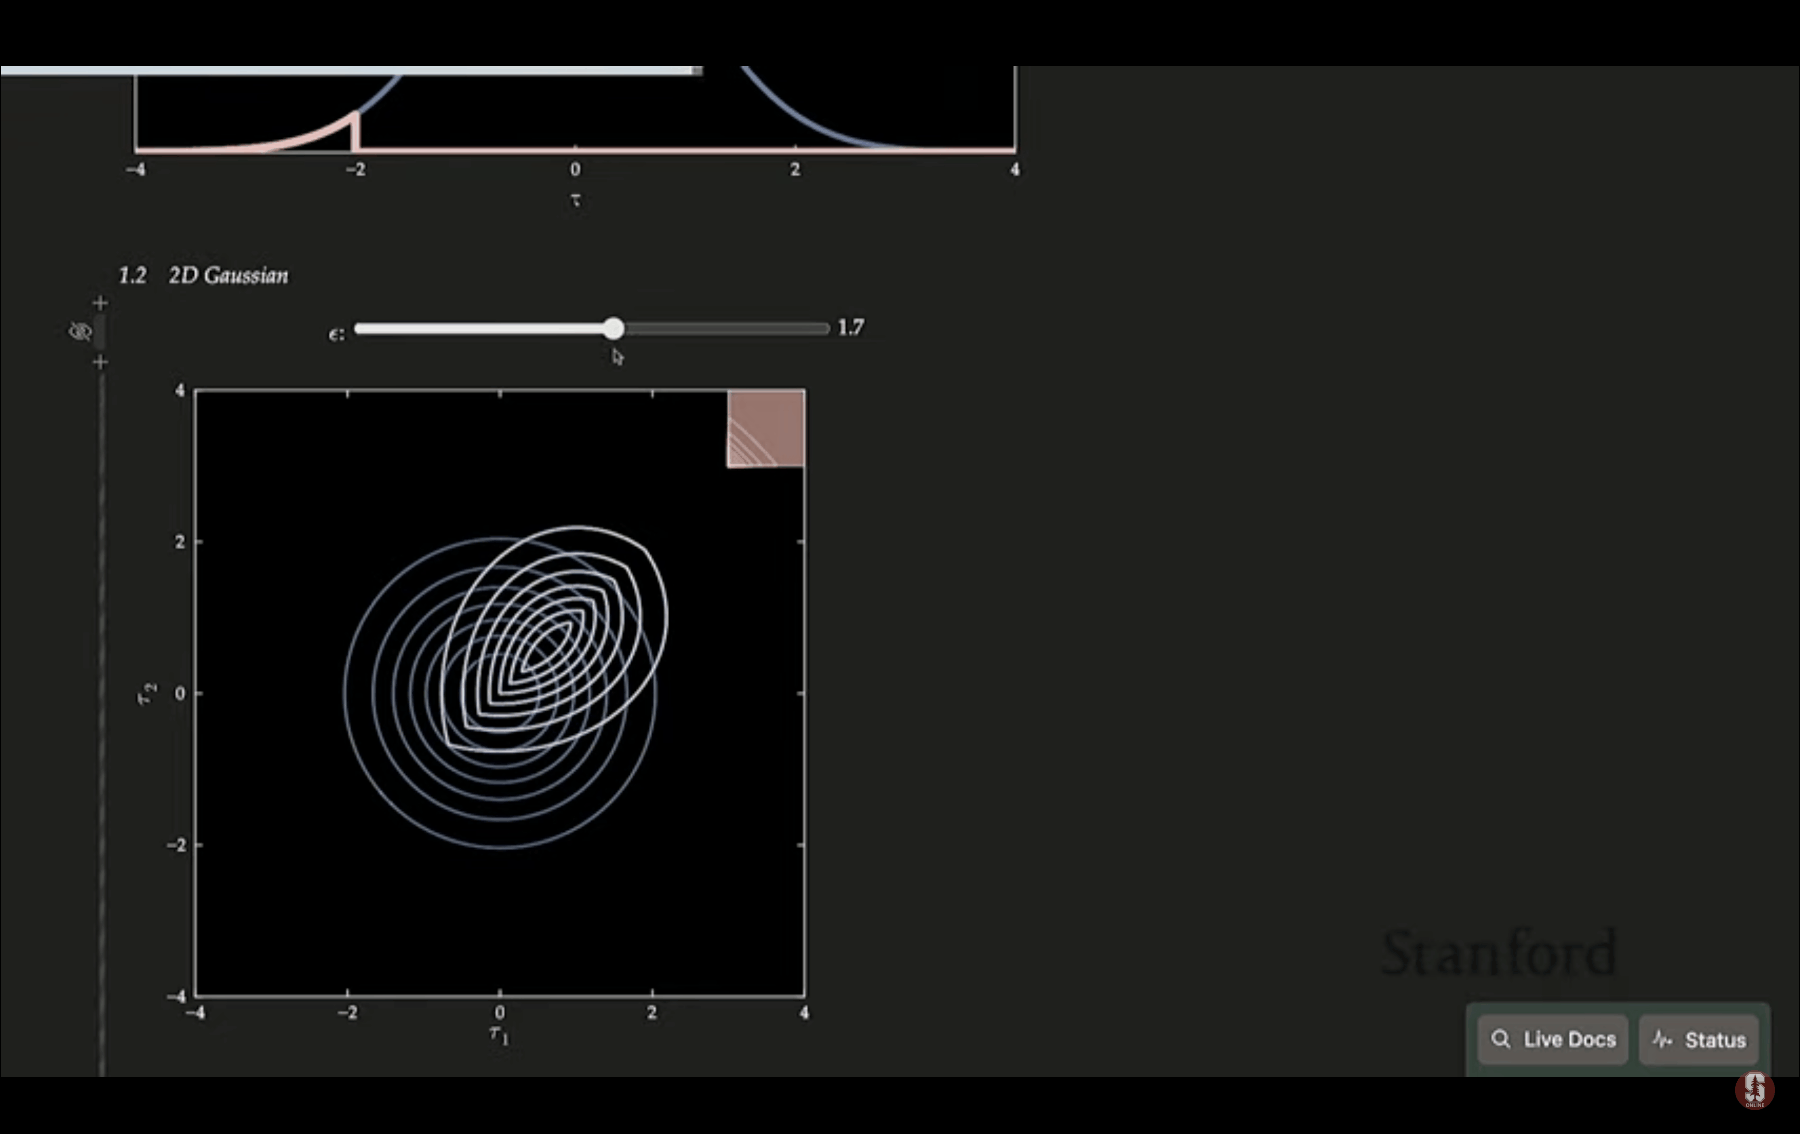
\includegraphics[width=0.7\linewidth]{media/aa228v-pluto-example.png}

{\footnotesize Interactive lectures using \jlv{Pluto.jl}}

\end{frame}
\begin{frame}[fragile]{Assignments in Julia} \pause

\begin{columns}
  \begin{column}{0.45\textwidth}
    \centering
    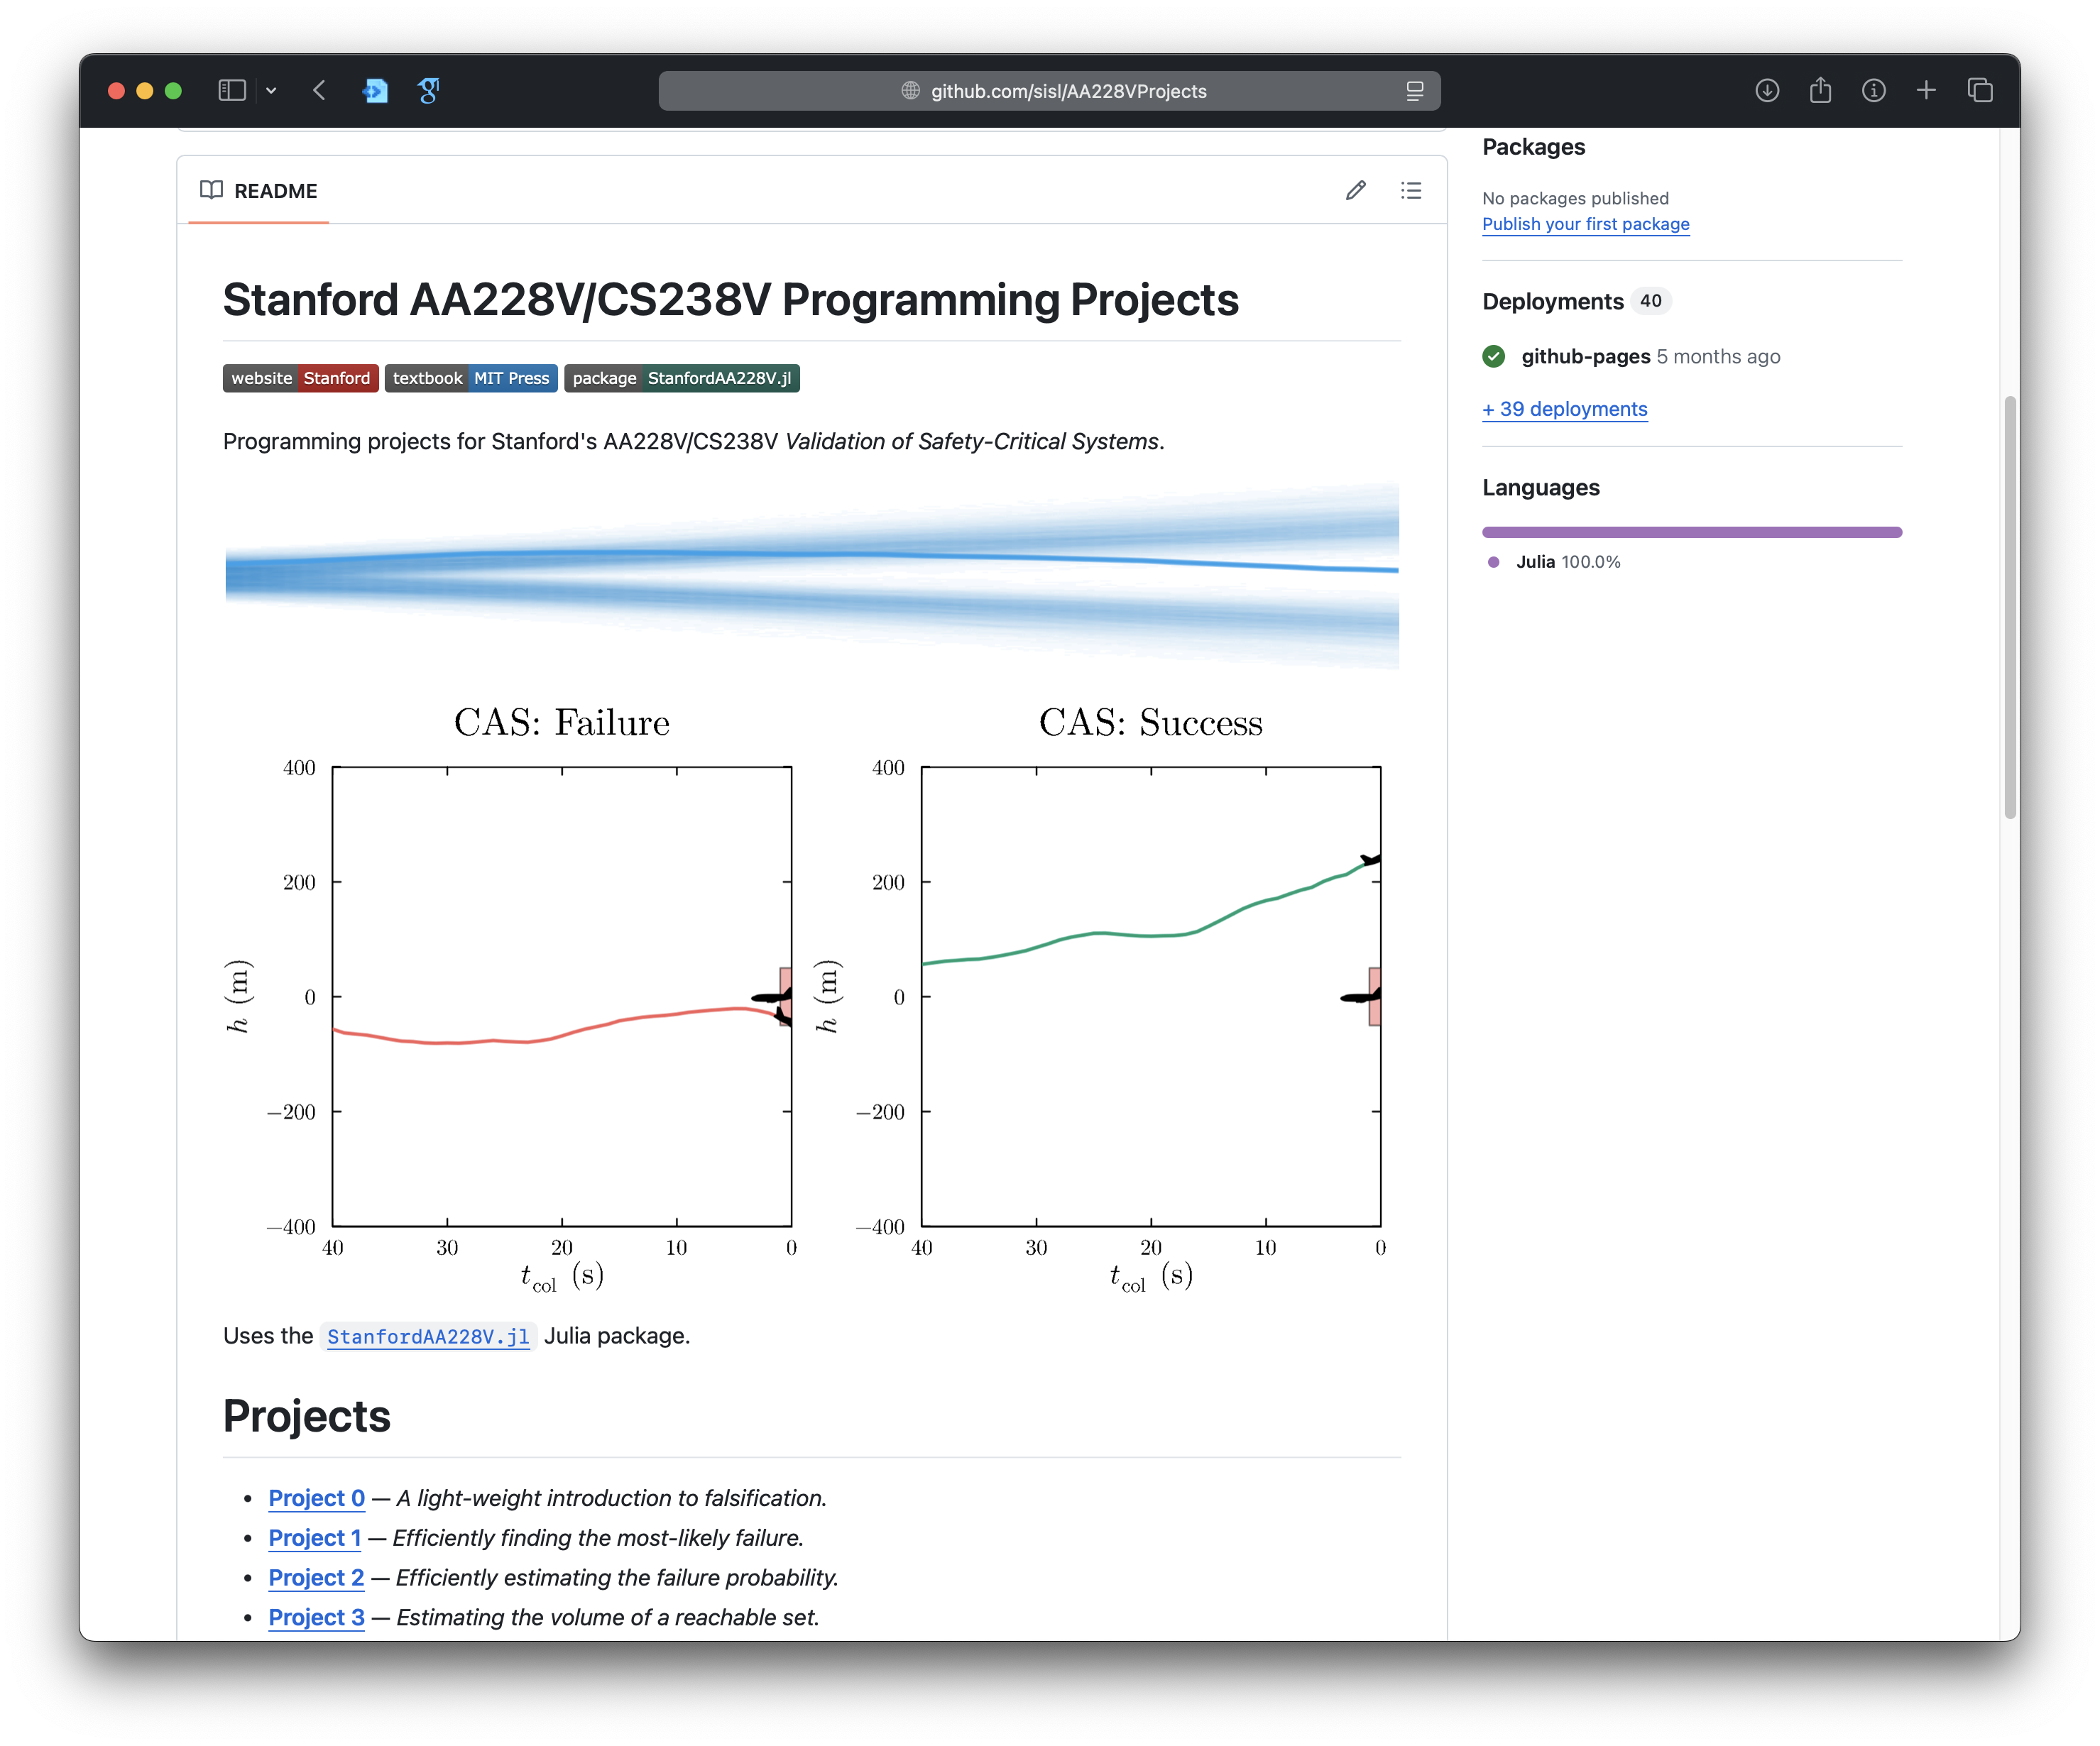
\includegraphics[width=\linewidth]{media/AA228VProjects.png}

    \captionof*{figure}{\shortstack{\footnotesize Assignments repository\\\textcolor{gray}{\scriptsize Student-facing code}}}
  \end{column}
  \pause
  \begin{column}{0.45\textwidth}
    \centering
    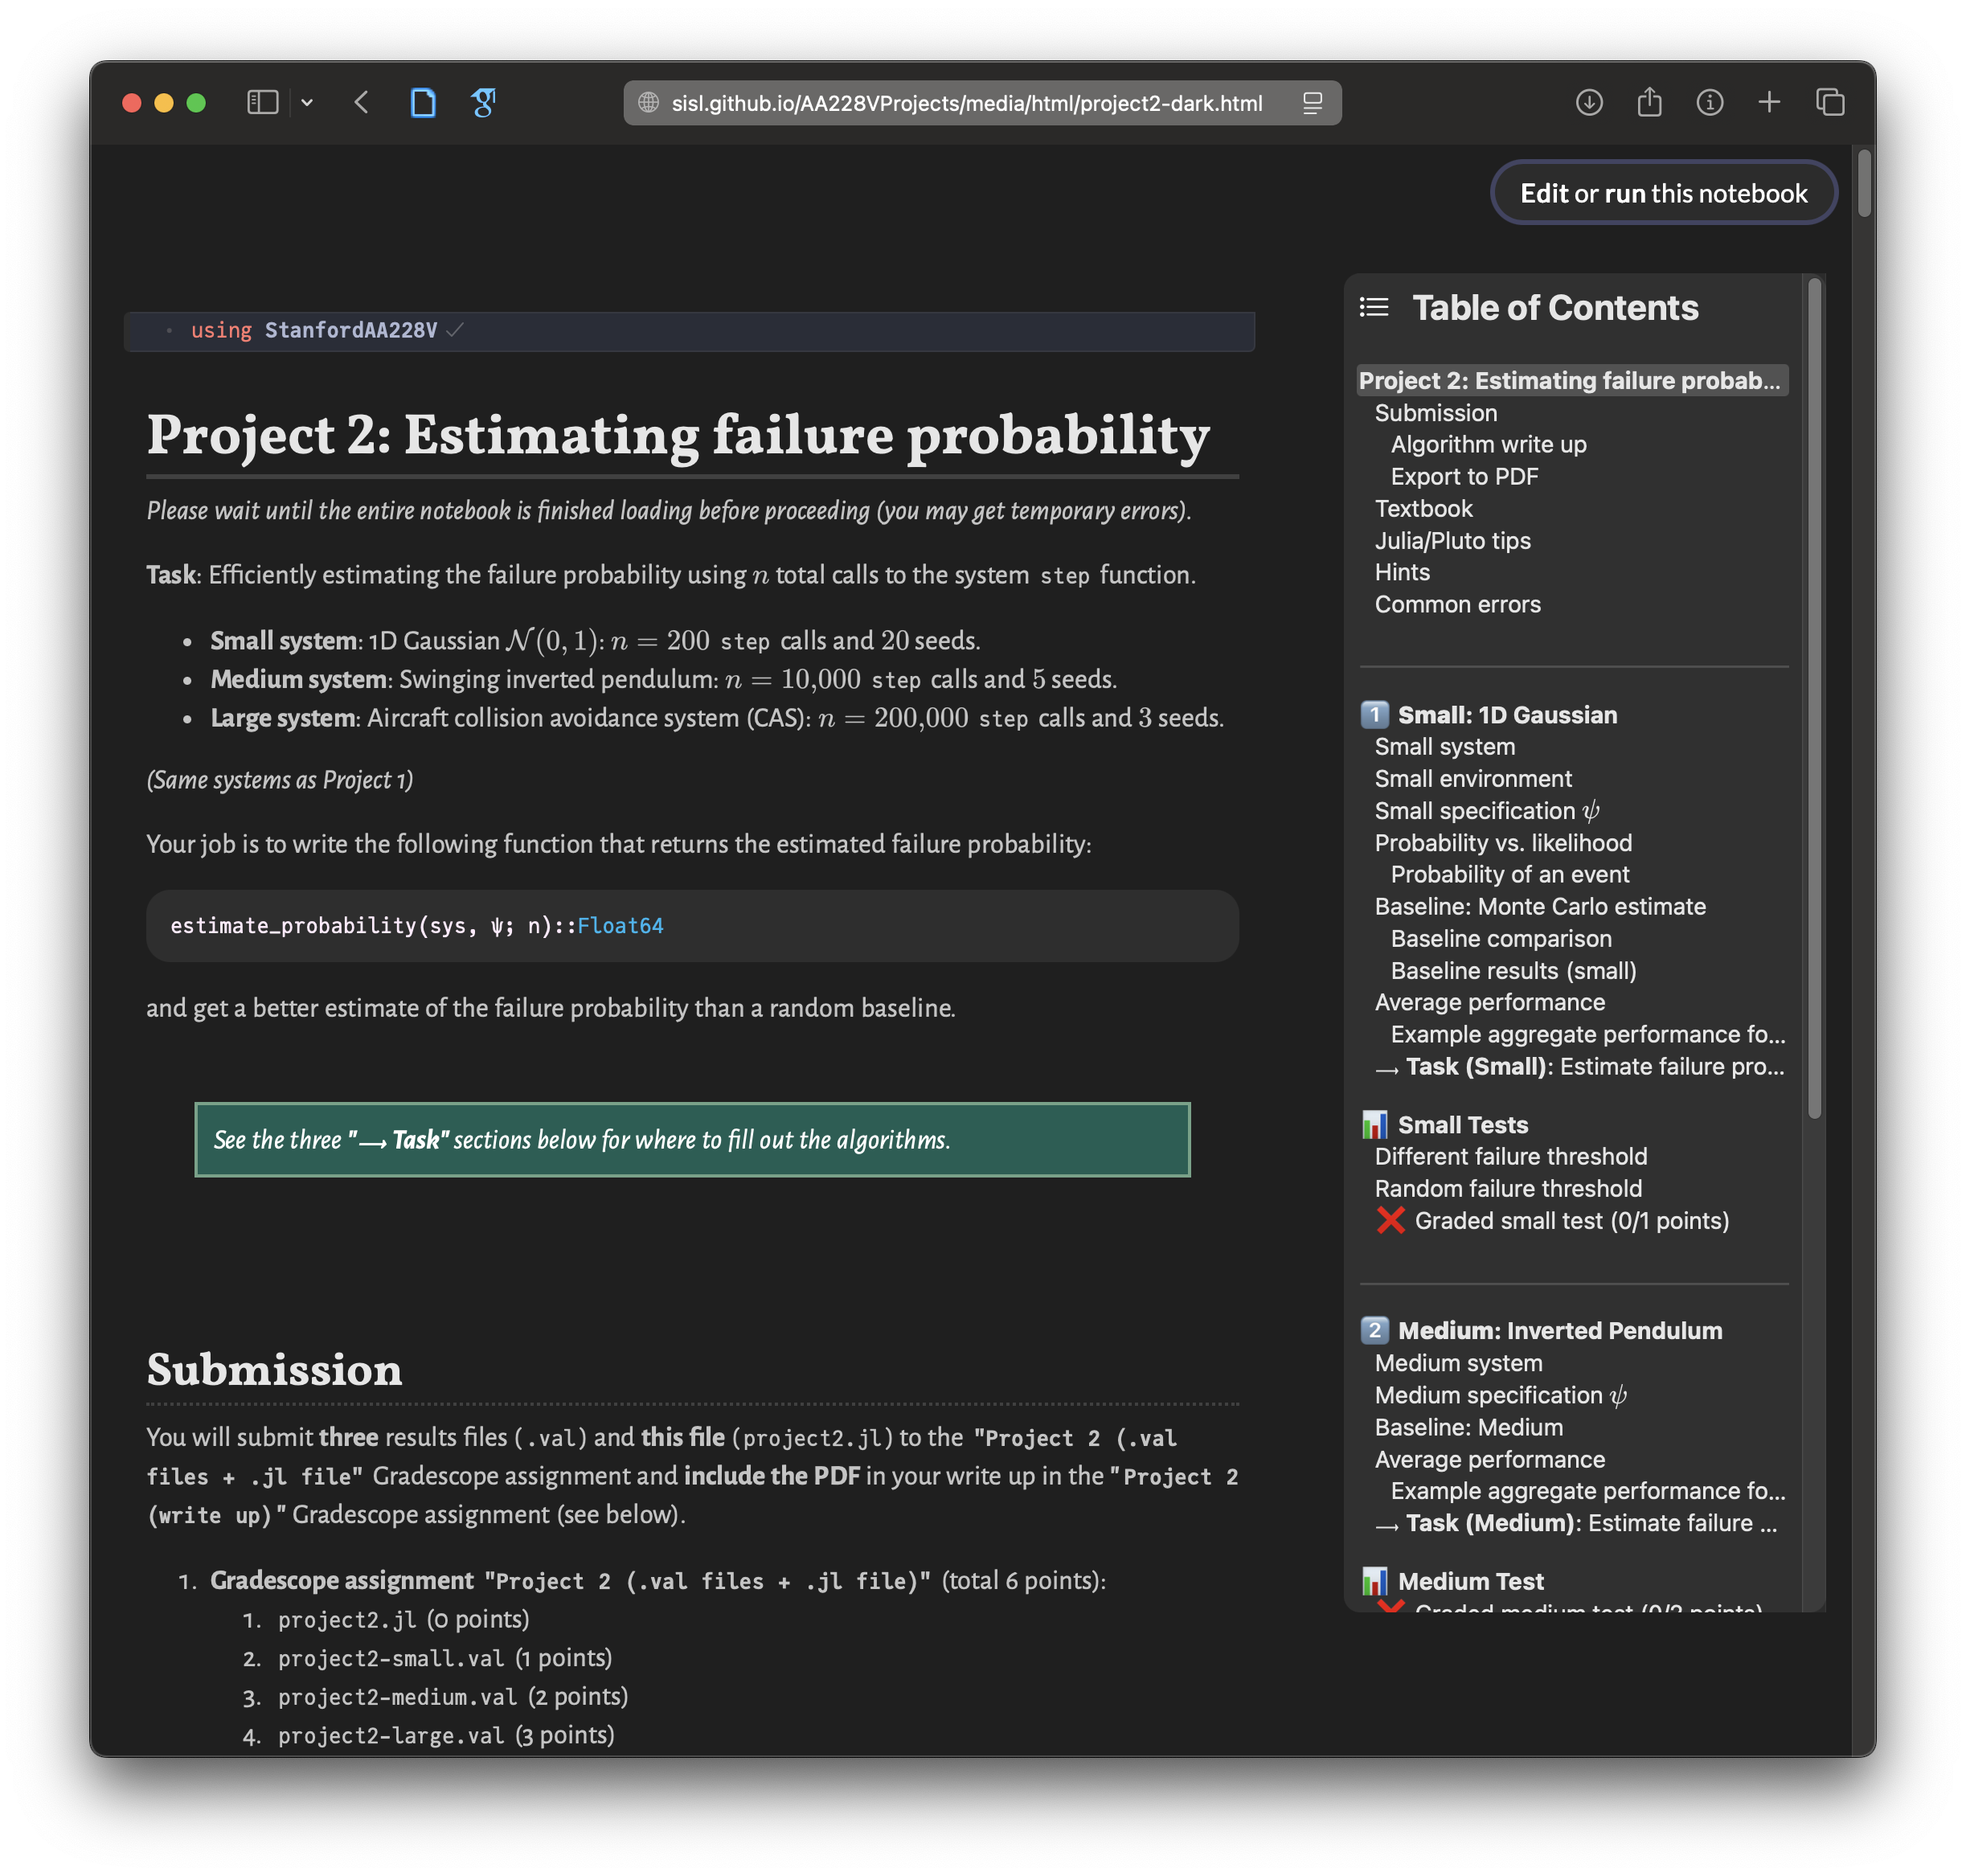
\includegraphics[width=\linewidth]{media/project2.png}

    \captionof*{figure}{\shortstack{\footnotesize Pluto assignments\\\textcolor{gray}{\scriptsize Includes local tests}}}
  \end{column}
  \hfill
\end{columns}

\end{frame}


\begin{frame}[fragile]{Assignments in Julia}

\begin{columns}
  \hfill
  \begin{column}{0.45\textwidth}
    \centering
    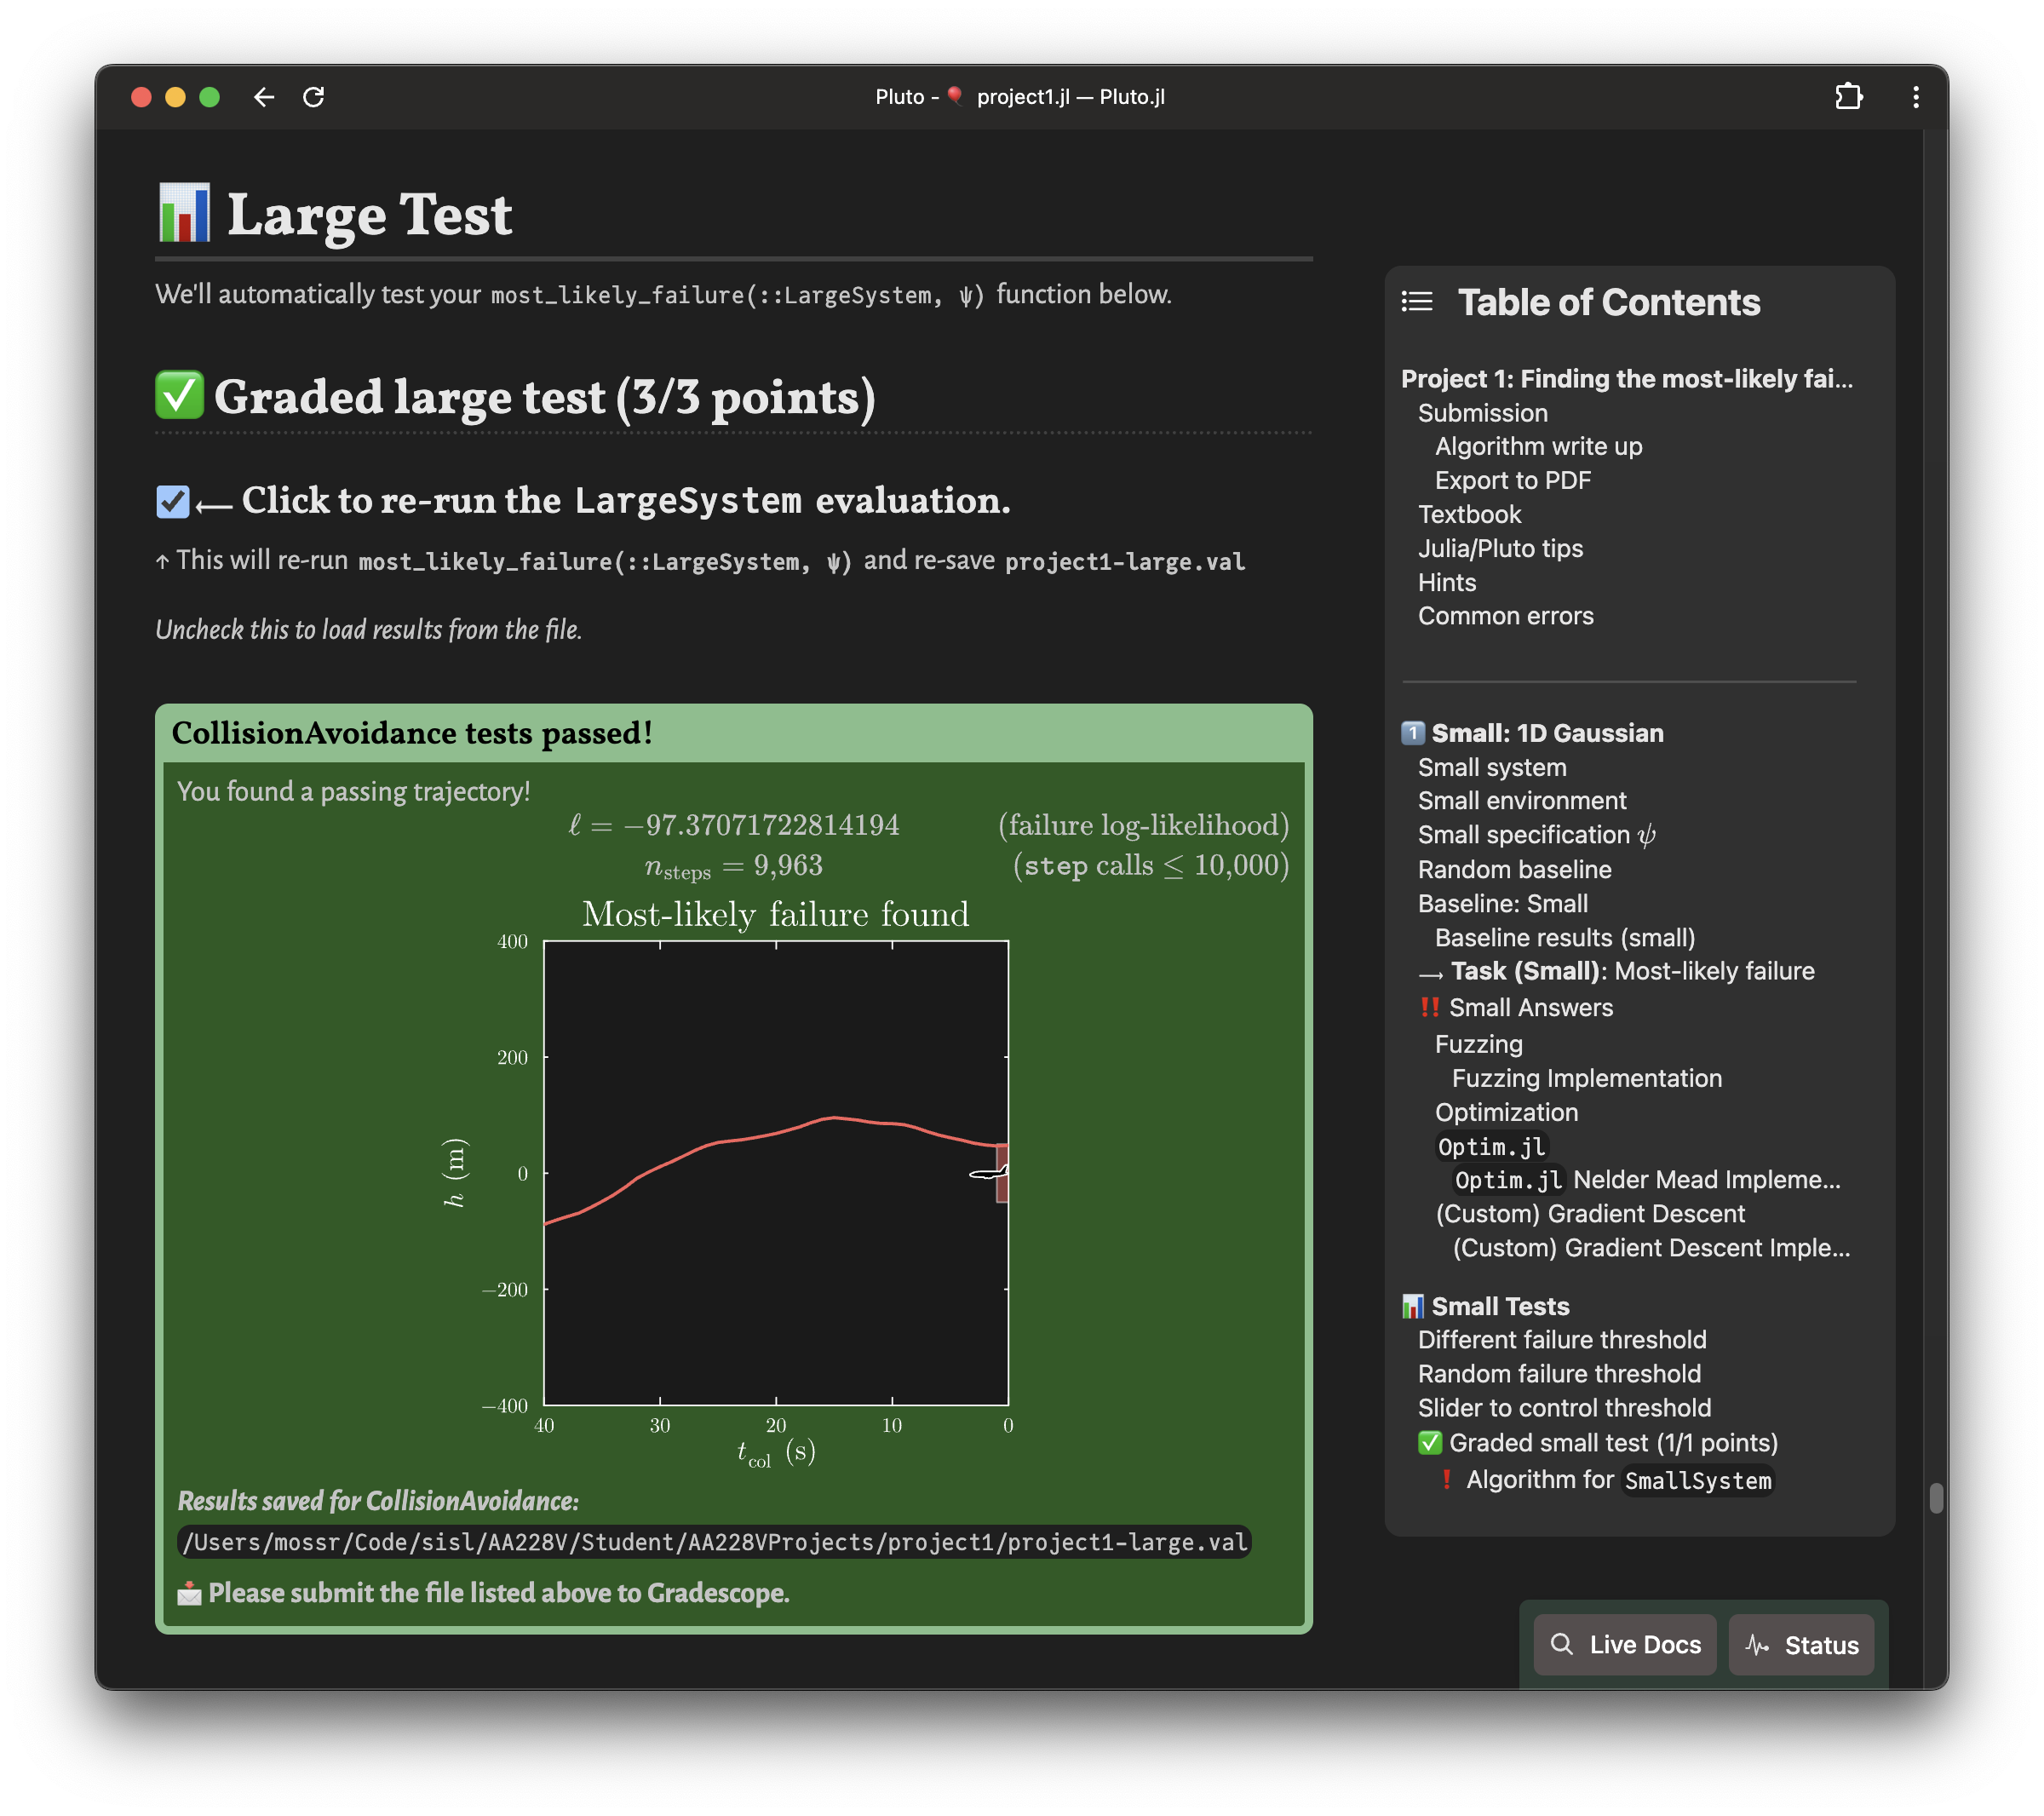
\includegraphics[width=\linewidth]{media/project1.png}

    \captionof*{figure}{\shortstack{\footnotesize Interactive Pluto assignments\\\textcolor{gray}{\scriptsize Get feedback instantly}}}
  \end{column}
  \pause
  \begin{column}{0.54\textwidth}
    \small
    \begin{itemize}
      \item Separated assignment code from core library (\jlv{StanfordAA228V.jl}) \pause
      \item Interactive nature allows students to play with their algorithms \pause
      \item No ``hidden state'' that may confuse students \pause
      \item Open-source nature requires clever obfuscation of solution code \pause
      \item Metaprogramming serves as lightweight way to track and enforce student requirements \pause
      \item Local tests exactly match graded tests \pause
    \end{itemize}
  \end{column}
  \hfill
\end{columns}

\end{frame}
\begin{frame}[fragile]{Grading Assignments} \pause

\begin{columns}
  \hfill
  \begin{column}{0.45\textwidth}
    \centering
    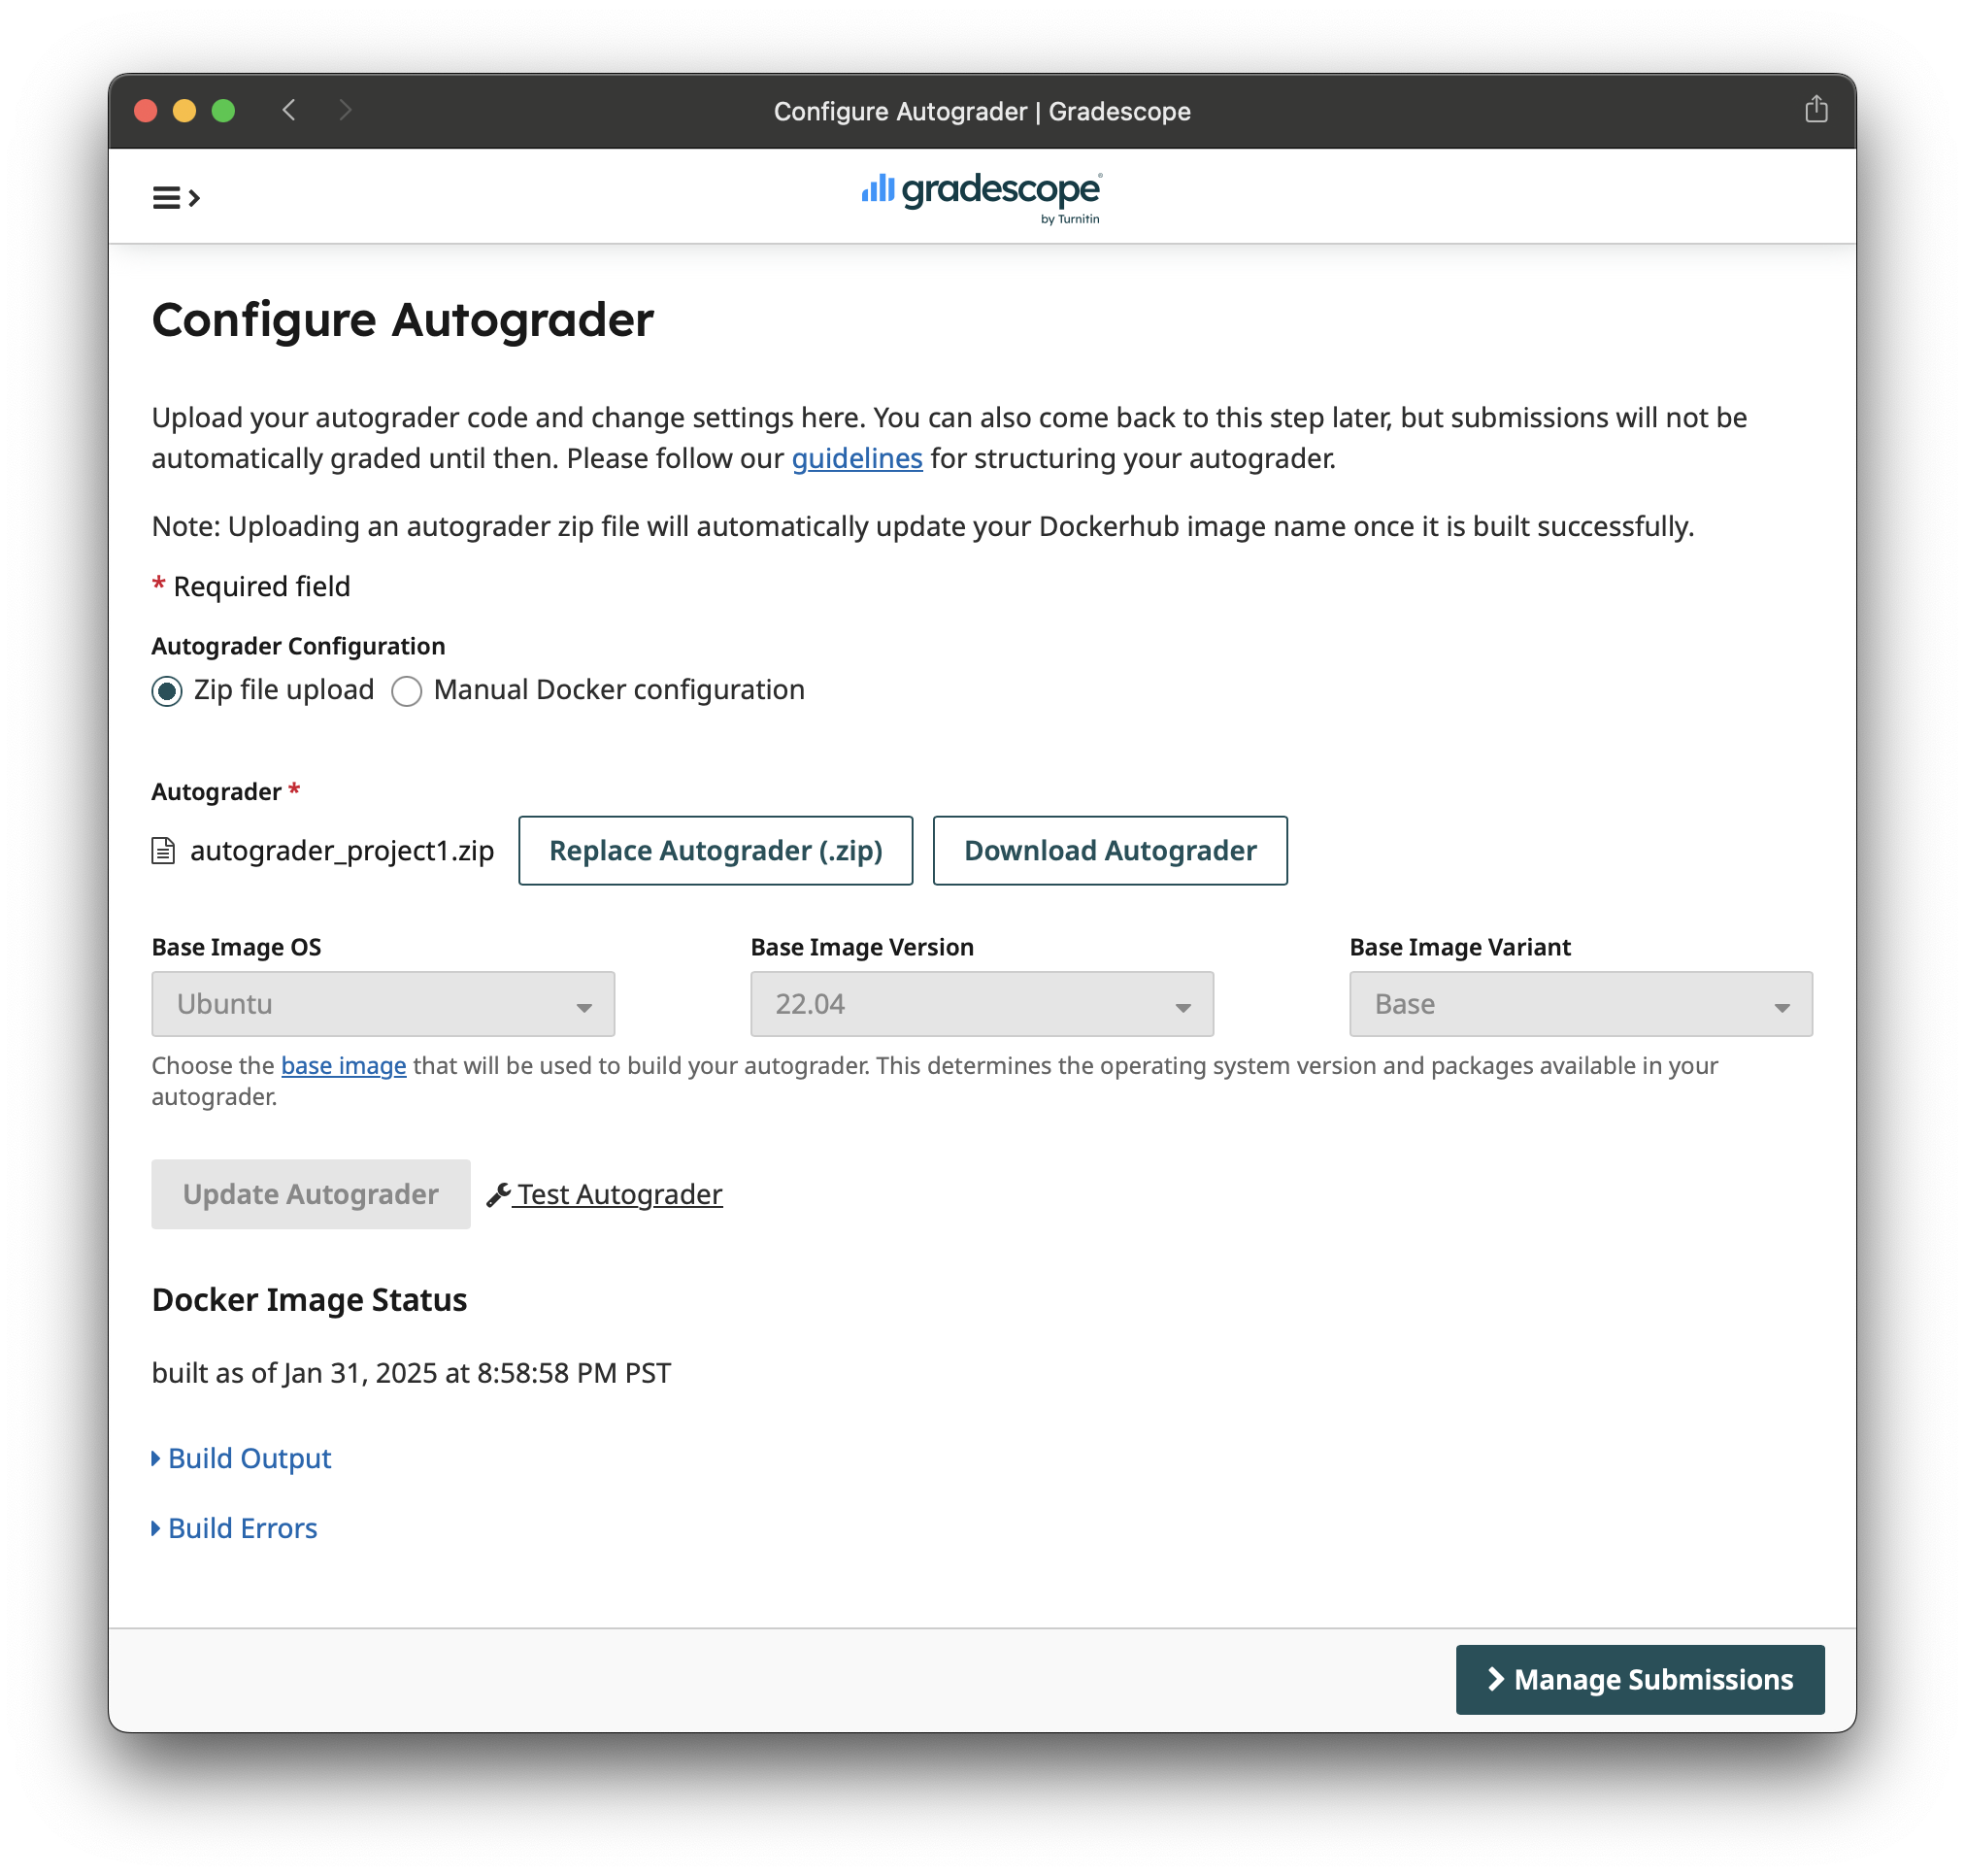
\includegraphics[width=\linewidth]{media/gradescope.png}

    \captionof*{figure}{\shortstack{\footnotesize Autograde via Gradescope\\\textcolor{gray}{\scriptsize Students upload Pluto notebook}}}
  \end{column}
  \pause
  \begin{column}{0.45\textwidth}
    \centering
    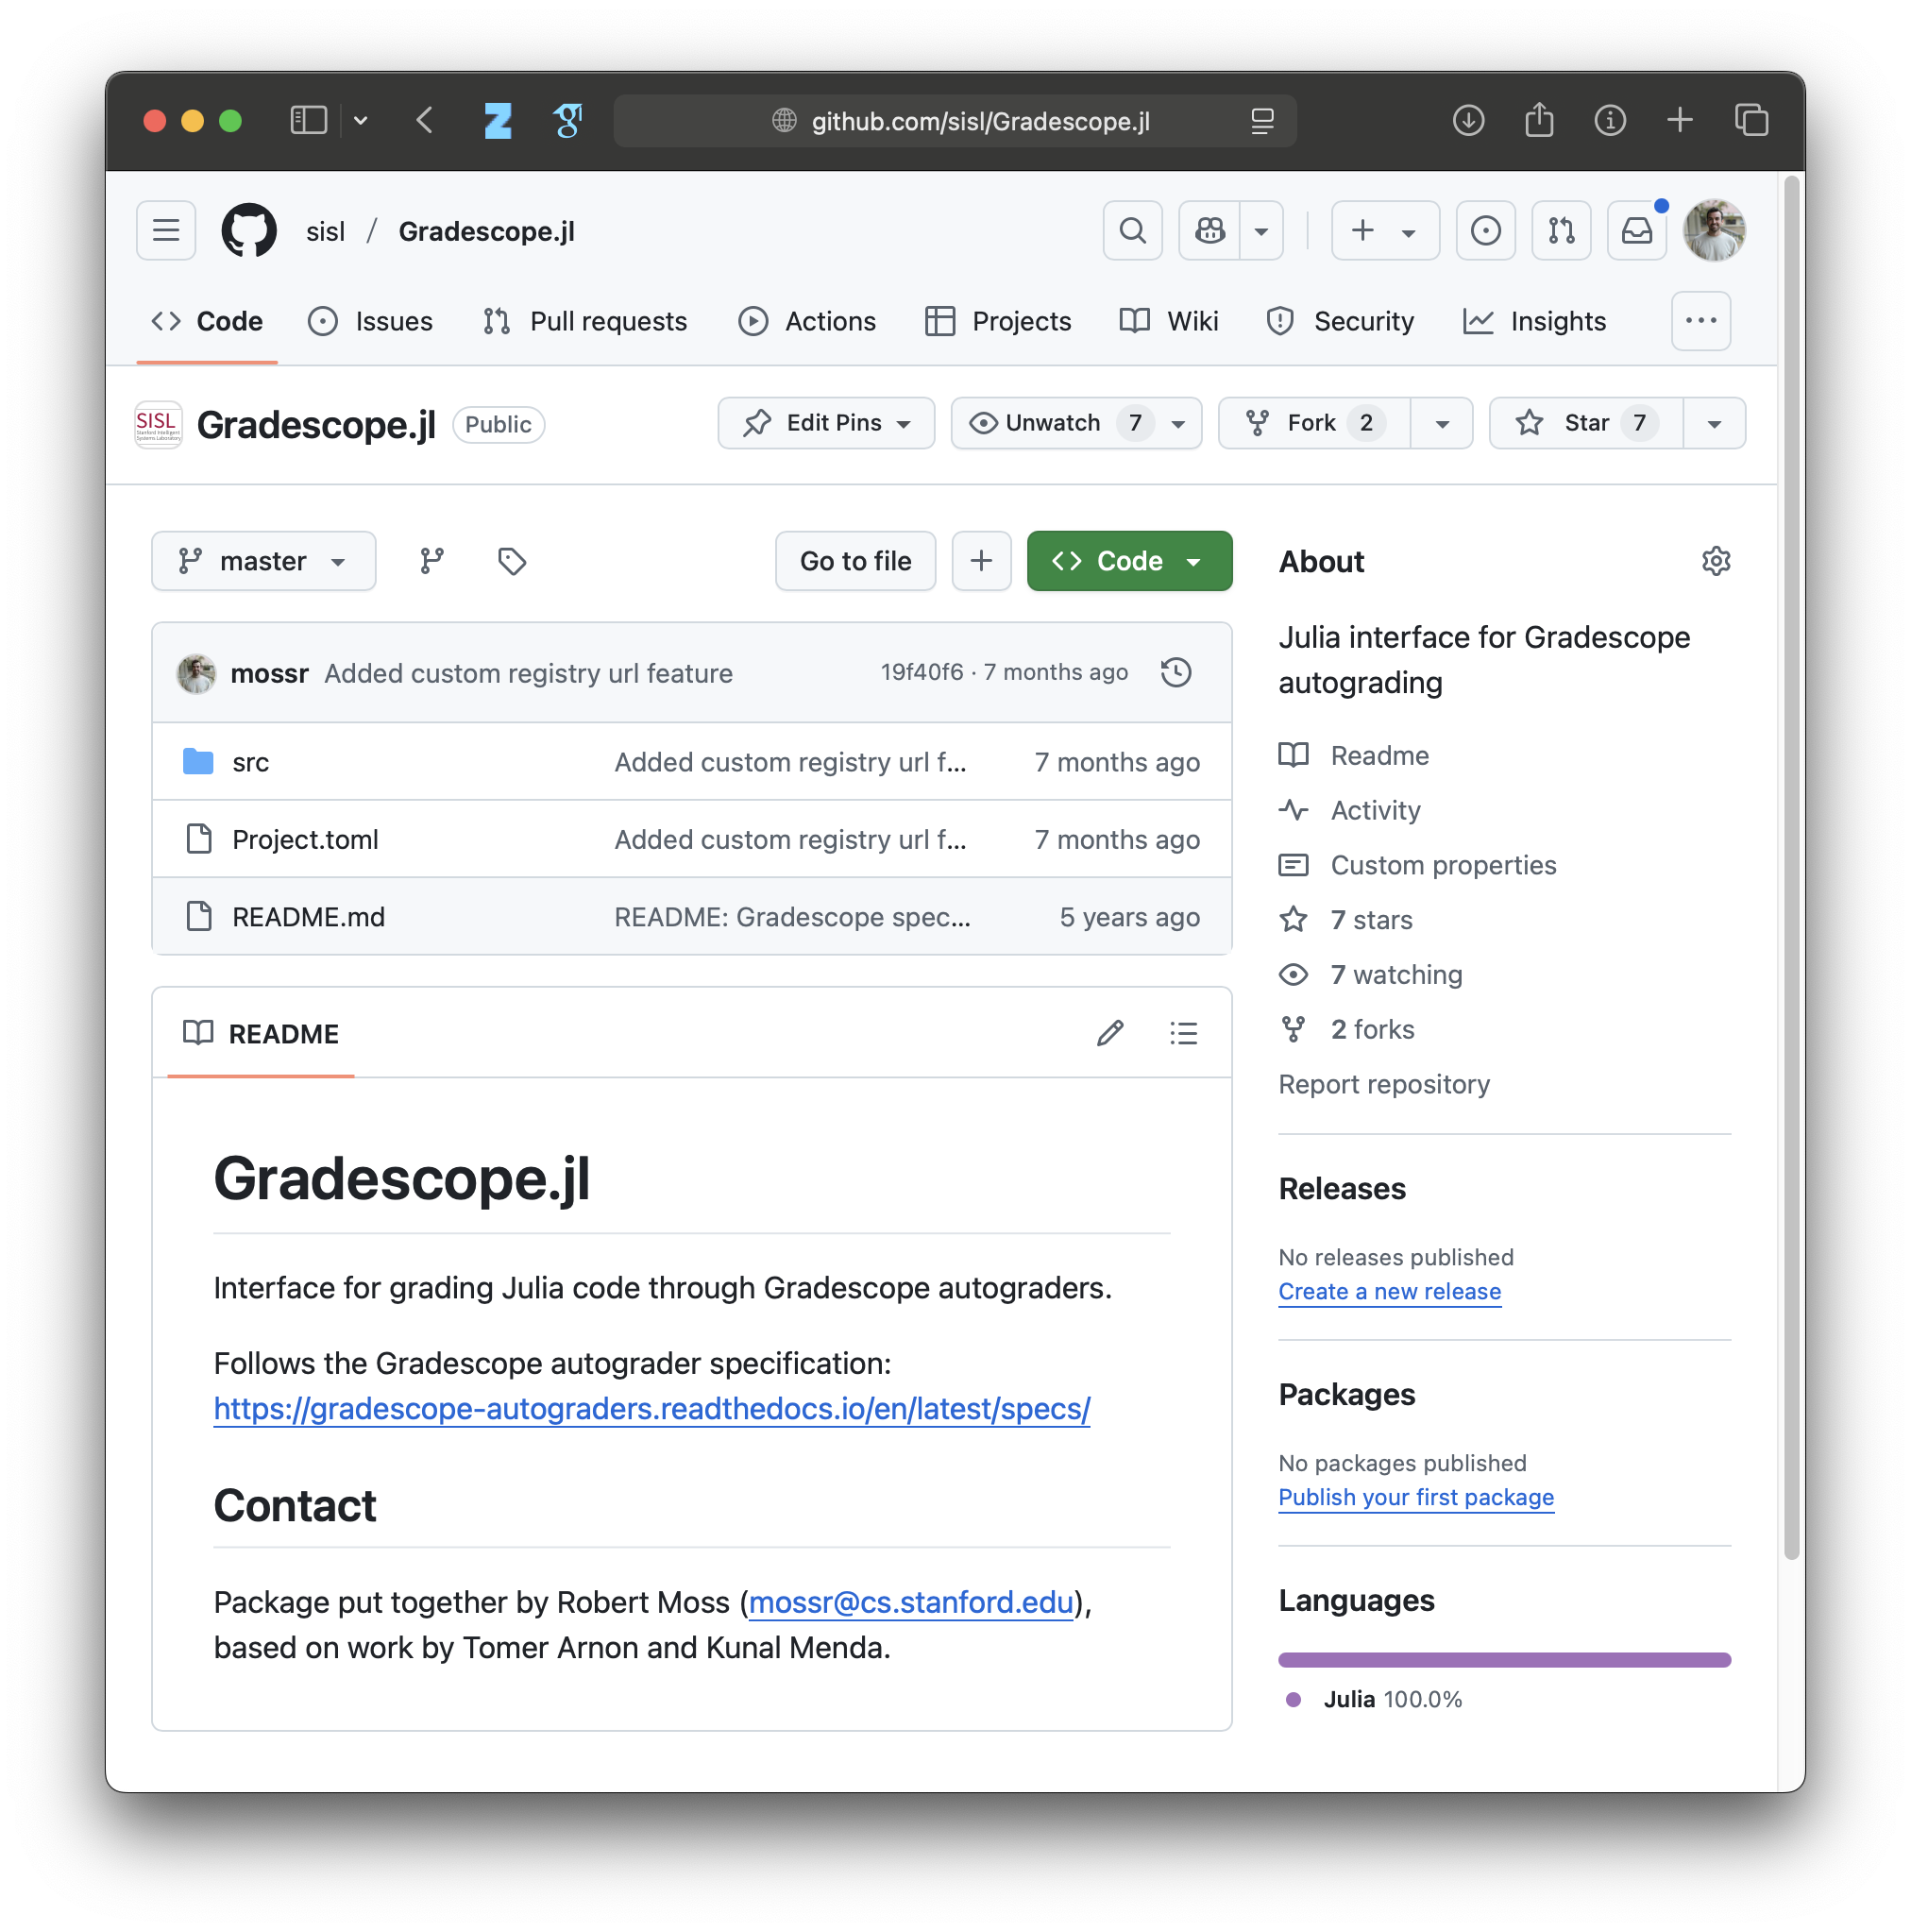
\includegraphics[width=\linewidth]{media/gradescope-jl.png}
    
    \captionof*{figure}{\shortstack{\footnotesize Light-weight \jlv{Gradescope.jl} package\\\textcolor{gray}{\scriptsize Manage deps and create autograders}}}
  \end{column}
  \hfill
\end{columns}

\end{frame}
\begin{frame}[fragile]{Future use of Julia in Academia} \pause

\begin{itemize}
    \item Teach fundamentals like probability and statistics in pure Julia \pause
    \item Unify curriculum across compounding courses \pause
    \item Build cohesive teaching materials using Pluto (e.g., through JuliaAcademy) \pause
    \item Build general grading frameworks to work across courses \pause
    \item Compile Julia code to binaries to avoid obfuscation \pause
    \item Write interactive research papers in Julia/Pluto
\end{itemize}

\end{frame}
\begin{frame}[fragile]{\normalfont\jlv{PlutoPapers.jl}} \pause

\centering
\textit{What if we could interact directly with the code in research papers?}

\end{frame}


\begin{frame}[fragile]{\normalfont\jlv{PlutoPapers.jl}}

\begin{columns}
  \hfill
  \begin{column}{0.35\textwidth}
    \centering
    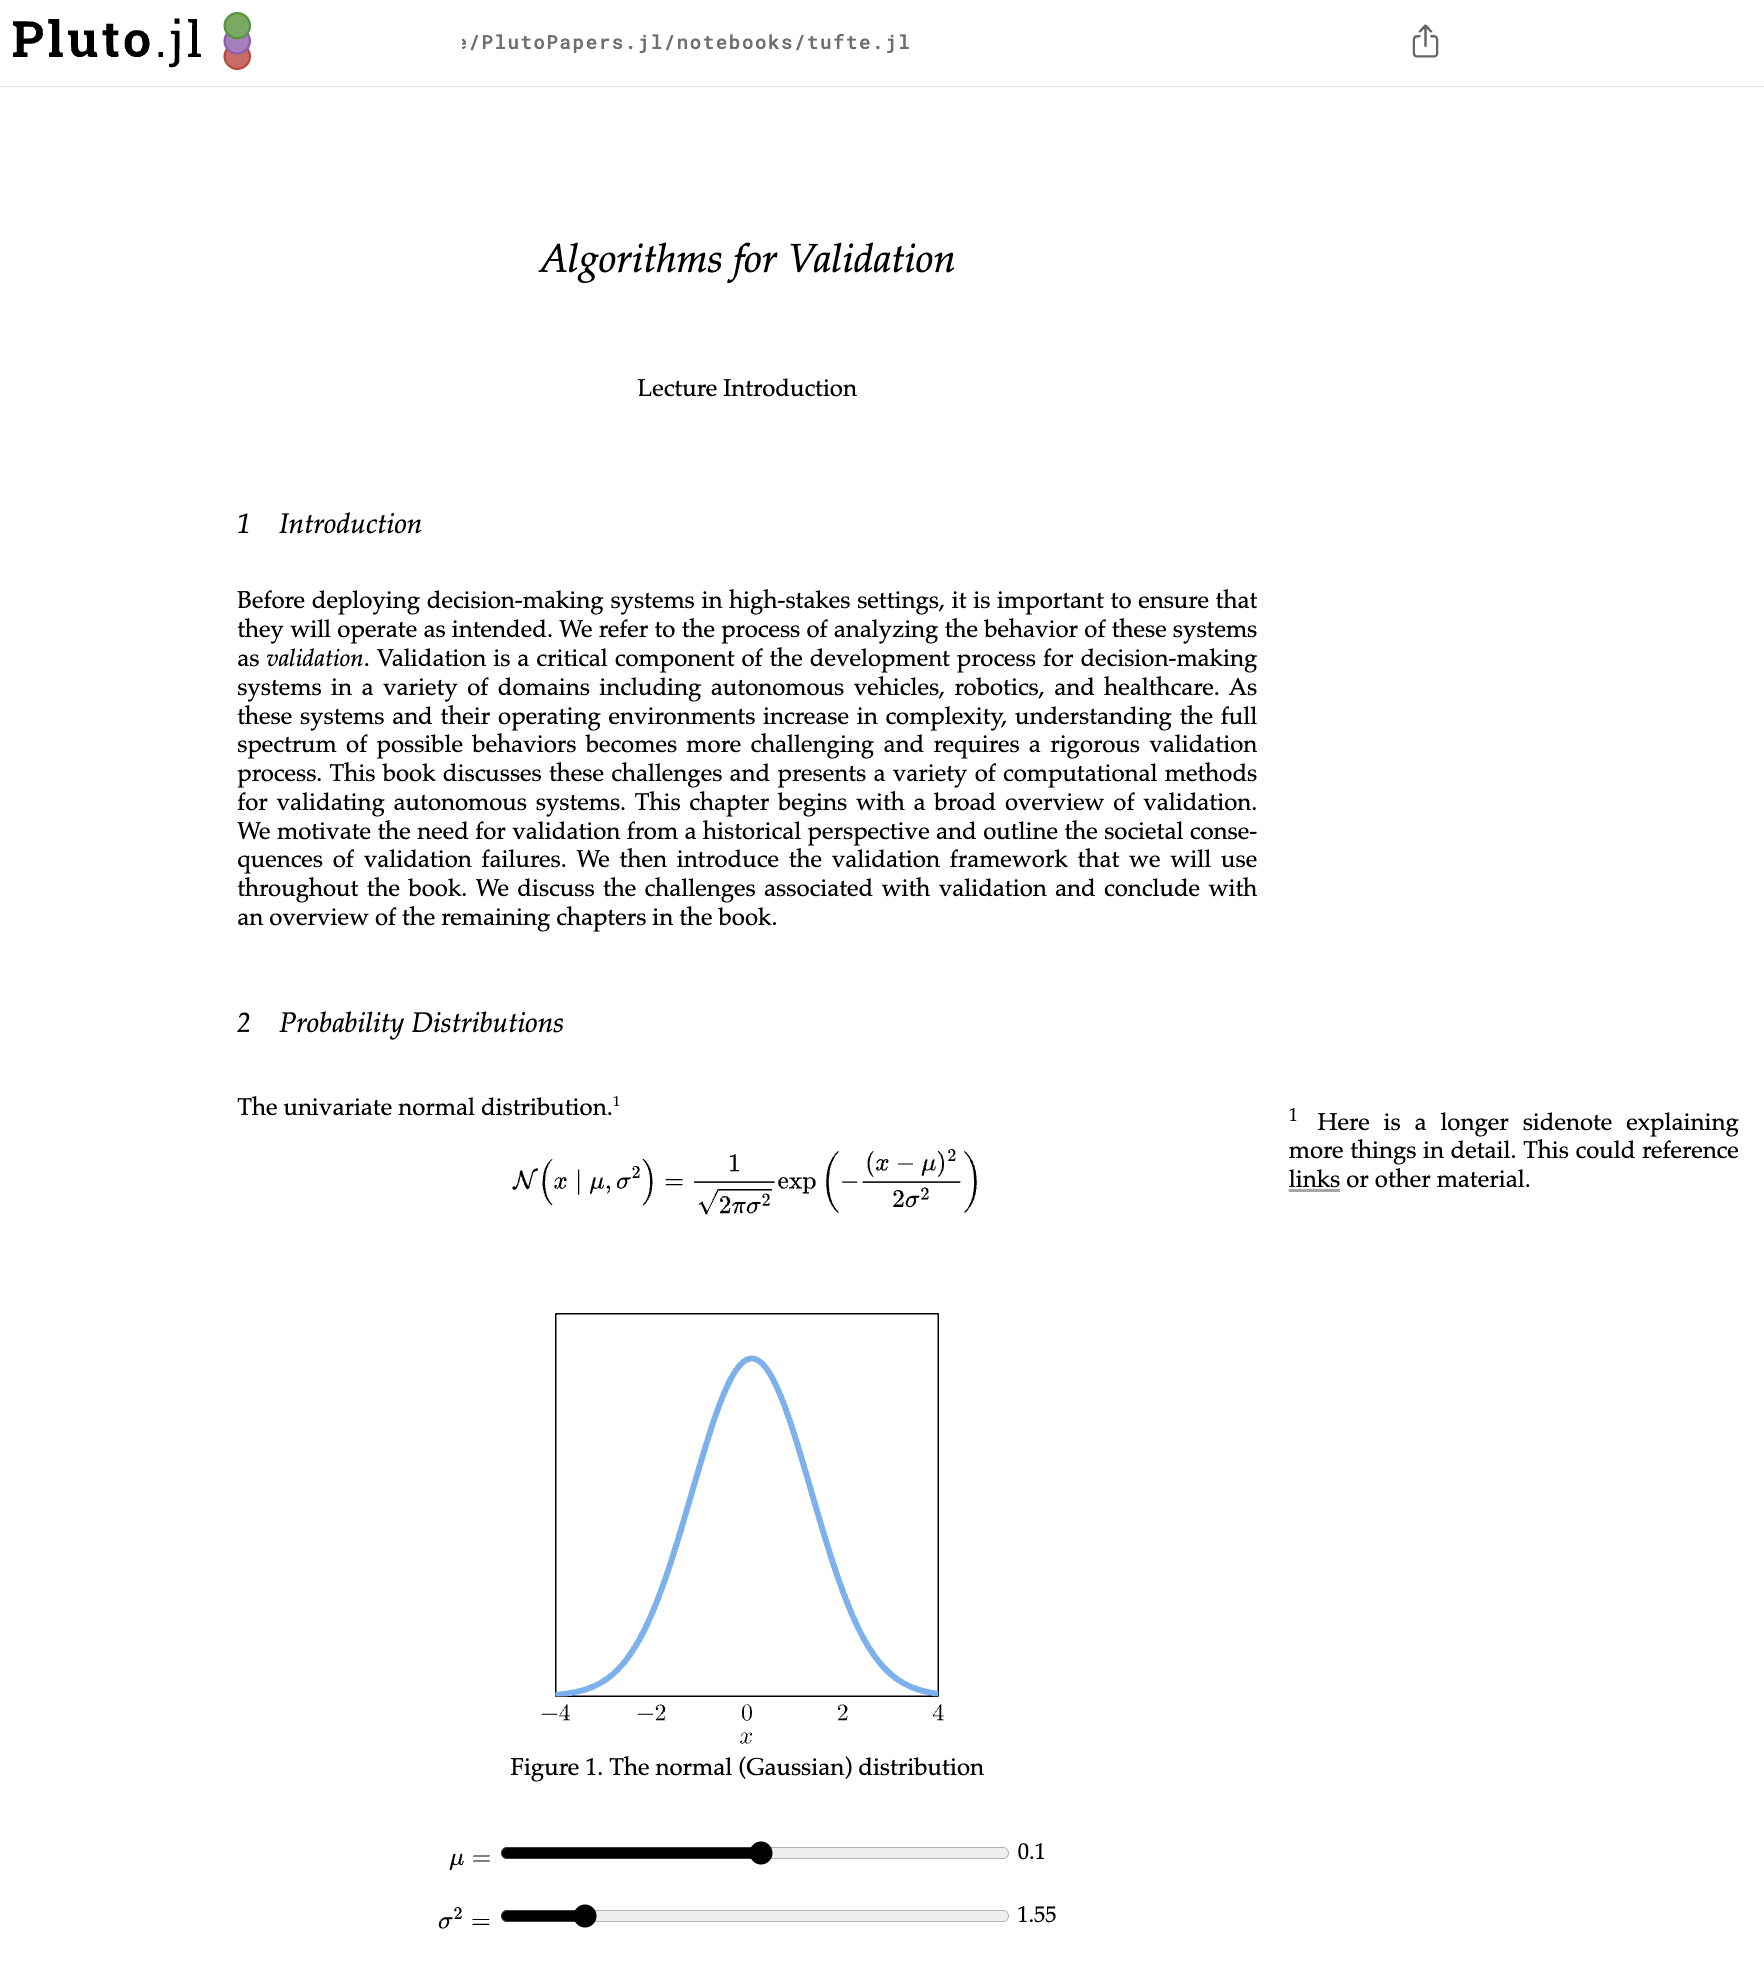
\includegraphics[width=\linewidth]{media/plutopapers-tufte-light.png}

    \captionof*{figure}{\shortstack{\footnotesize Interactive research papers\\\textcolor{gray}{\scriptsize Run code directly in the paper}}}
  \end{column}
  \pause
  \begin{column}{0.54\textwidth}
    
\includegraphics[width=0.85\linewidth]{media/PlutoPapers.jl.png}

    \textcolor{repo}{\small \url{https://github.com/mossr/PlutoPapers.jl}}
  \end{column}
  \hfill
\end{columns}
    
\end{frame}
\begin{frame}[fragile]{Thank you!}

\centering


\includegraphics[width=0.25\linewidth]{media/qr-code.png}

\phantom{---}

\Large
\textsc{Questions?}

\textcolor{gray}{\small\texttt{mossr@cs.stanford.edu}}
    
\end{frame}

\end{document}

% TODO: albatian
\usefonttheme{serif}
\usefonttheme{professionalfonts}
\usepackage{mathtools}
\usepackage[tracking=true]{microtype}

\usepackage{bold-extra}
\usepackage{realscripts}
\usepackage{amsmath,bm,amssymb}
\usepackage{amsthm}
\usepackage{bbm}
\usepackage{tikz}
\usepackage[group-digits=integer,group-minimum-digits=4,group-separator={,},detect-all]{siunitx}
\usepackage{algorithmicx}
\usepackage{algorithm}
\usepackage[noend]{algpseudocode}
\usepackage{xcolor}
\usepackage{multirow}
\usepackage{longtable,tabularx,booktabs}
\usepackage[flushleft]{threeparttable}
\usepackage{vector} % local
\usepackage{varwidth}
\usepackage{fancyvrb}
\usepackage{tcolorbox}
\usepackage{ifthen}
\usepackage{pagecolor}
\usepackage{textpos}
\usepackage{calc}
\usepackage{adjustbox}

%%%%%%%%%%%%%%%%%%%%%%%%%%%%%%%%%%%%%%%%%%%%%%%%%%
% Unicode settings
%%%%%%%%%%%%%%%%%%%%%%%%%%%%%%%%%%%%%%%%%%%%%%%%%%
% \setmonofont{DejaVu Sans Mono}[Scale=MatchLowercase]
% \usepackage{newunicodechar}
% \newfontface{\calligraphic}{Latin Modern Math}[Scale=0.85]

% https://juliamono.netlify.app/faq/#can_i_use_it_in_a_latex_document
\setmonofont{JuliaMono-Regular}[
	UprightFont = JuliaMono-Medium,
	BoldFont = JuliaMono-ExtraBold,
	ItalicFont = JuliaMono-Light,
    Contextuals = Alternate,
    Scale = MatchLowercase,
    Path = ./fonts/,
    Extension = .ttf
]

% Remove empty lines in juliaconsole
% https://github.com/gpoore/pythontex/issues/98#issuecomment-318078264
\makeatletter
\AtBeginEnvironment{juliaconsole}{%
  \def\FV@@PreProcessLine{%
    \expandafter\ifstrempty\expandafter{\FV@Line}{}{%
      \FV@StepLineNo
      \FV@Gobble
      \expandafter\FV@ProcessLine\expandafter{\FV@Line}}}%
}
\makeatother


%%%%%%%%%%%%%%%%%%%%%%%%%%%%%%%%%%%%%%%%%%%%%%%%%%
% Reference (biber) settings
%%%%%%%%%%%%%%%%%%%%%%%%%%%%%%%%%%%%%%%%%%%%%%%%%%
\usepackage[style=verbose,backend=biber]{biblatex}
% \addbibresource{preamble/main.bib}
\addbibresource{\jobname.bib}
% \setbeamerfont{footnote}{size=\tiny}
\setbeamerfont{footnote}{size=\fontsize{4}{5}\selectfont}
\setbeamertemplate{bibliography item}{}% Remove reference icon.
\renewcommand*{\bibfont}{\footnotesize}


%%%%%%%%%%%%%%%%%%%%%%%%%%%%%%%%%%%%%%%%%%%%%%%%%%
% Colors
%%%%%%%%%%%%%%%%%%%%%%%%%%%%%%%%%%%%%%%%%%%%%%%%%%
\ifdefined\INVERTED
    \pagecolor{black} % Comment out to hide background
    \colorlet{primarycolor}{white}
    \colorlet{secondarycolor}{black}
    \colorlet{shadecolor}{black!85}
    \definecolor{cardinal}{HTML}{B83A4B}
    \definecolor{coolgrey}{HTML}{767674}
    \definecolor{captioncolor}{HTML}{59B3A9}
    \definecolor{captionsecondarycolor}{HTML}{2D716F}
    \colorlet{pagecolor}{lightgray}
    \colorlet{algbgcolor}{darkgray}
\else
    \colorlet{primarycolor}{black}
    \colorlet{secondarycolor}{white}
    \colorlet{shadecolor}{black!5}
    \definecolor{cardinal}{HTML}{8C1515}
    \definecolor{coolgrey}{HTML}{53565A}
    % \definecolor{captioncolor}{HTML}{3333B2} % Blue
    % \definecolor{captionsecondarycolor}{HTML}{7A7ACD} % Light blue
    \definecolor{captioncolor}{HTML}{59B3A9}
    \definecolor{captionsecondarycolor}{HTML}{2D716F}
    \colorlet{pagecolor}{darkgray}
    \colorlet{algbgcolor}{lightgray}
\fi

\definecolor{darkgreen}{RGB}{21,140,21}
\definecolor{darkblue}{RGB}{21,21,140}
\definecolor{sun}{RGB}{234,171,0}

\newcommand{\darkblue}[1]{{\color{darkblue} #1}}
\newcommand{\darkgreen}[1]{{\color{darkgreen} #1}}
\newcommand{\darkred}[1]{{\color{cardinal} #1}}

% Colorblind-Friendly Color Scheme
% A compromise between the original colorscheme and
% this palette: https://www.nature.com/articles/nmeth.1618
\definecolor{pastelMagenta}{HTML}{FF48CF} % magenta
\definecolor{pastelPurple}{HTML}{8770FE} % purple
\definecolor{pastelBlue}{RGB}{0,114,178} % blue 0072B2
\definecolor{pastelSkyBlue}{RGB}{86,180,233} % sky blue 56B4E9
\definecolor{pastelGreen}{RGB}{0,158,115} % green 009E73
\definecolor{pastelOrange}{RGB}{230,159,0} % orange E69F00
\definecolor{pastelRed}{HTML}{F5615C} % red
\definecolor{darkColor}{HTML}{300A24} % dark
\definecolor{pastelGreenBlue}{RGB}{43, 169, 174} % mix of pastelGreen and pastelSkyBlue

\newcommand{\colorPastelMagenta}{magenta}
\newcommand{\colorPastelPurple}{purple}
\newcommand{\colorPastelBlue}{blue}
\newcommand{\colorPastelSkyBlue}{sky blue}
\newcommand{\colorPastelGreen}{green}
\newcommand{\colorPastelOrange}{orange}
\newcommand{\colorPastelRed}{red}
\newcommand{\colorDark}{gray}


%%%%%%%%%%%%%%%%%%%%%%%%%%%%%%%%%%%%%%%%%%%%%%%%%%
% Beamer hide lines of code settings
%%%%%%%%%%%%%%%%%%%%%%%%%%%%%%%%%%%%%%%%%%%%%%%%%%
\tcbset{
  coloredbox/.style={
    colback=secondarycolor,
    colframe=secondarycolor,
    boxrule=0pt,
    width=\linewidth,
    sharp corners,
    height=0.83\baselineskip,
    % opacityback=0.5,
    before skip=0pt,
    after skip=0pt
  }
}

% Define a temporary length
\newlength{\testlen}
\newcommand{\lineblackout}[1]{%
    % Calculate the total shift: -\baselineskip - (N * 0.8)\baselineskip
    \pgfmathsetlength{\testlen}{-\baselineskip - #1 * 0.805\baselineskip}%
    \begin{textblock*}{\textwidth}(0cm, \testlen)
        \begin{tcolorbox}[standard jigsaw, coloredbox]\end{tcolorbox}
    \end{textblock*}
}


%%%%%%%%%%%%%%%%%%%%%%%%%%%%%%%%%%%%%%%%%%%%%%%%%%
% PGFPlot settings
%%%%%%%%%%%%%%%%%%%%%%%%%%%%%%%%%%%%%%%%%%%%%%%%%%
\usepackage{pgfplots}

\pgfplotsset{compat=newest}
\pgfplotsset{every axis legend/.append style={legend cell align=left, font=\footnotesize, draw=none, fill=none}}
\pgfplotsset{every axis/.append style={axis background/.style={fill=secondarycolor}}}
\pgfplotsset{every tick label/.append style={font=\footnotesize}}
\pgfplotsset{every axis label/.append style={font=\footnotesize}}

\fvset{baselinestretch=0.8}
\usepgfplotslibrary{fillbetween}
\usepgfplotslibrary{groupplots}
\usepgfplotslibrary{patchplots}
\usepgfplotslibrary{statistics}
\usepgfplotslibrary{ternary}


% NOTE: This won't work in Overleaf
\begin{jlcode}
  include("../../jl/support_code.jl")

  using Colors
  using ColorSchemes
  pasteljet = ColorMaps.RGBArrayMap(ColorSchemes.viridis, interpolation_levels=500, invert=true);
  pastelRedBlue = ColorMaps.RGBArrayMap([RGB(246/255, 21/255, 92/255),
                                         RGB(1.0,1.0,1.0),
                                         RGB( 27/255,161/255,234/255)], interpolation_levels=500);
\end{jlcode}


%%%%%%%%%%%%%%%%%%%%%%%%%%%%%%%%%%%%%%%%%%%%%%%%%%
% TikZ settings
%%%%%%%%%%%%%%%%%%%%%%%%%%%%%%%%%%%%%%%%%%%%%%%%%%
\usetikzlibrary{calc}
\usetikzlibrary{fit}
\usetikzlibrary{positioning}
\usetikzlibrary{arrows}
\usetikzlibrary{arrows.meta}
\usetikzlibrary{decorations.pathreplacing}
\usetikzlibrary{decorations.pathmorphing}
\usetikzlibrary{decorations.text}
\usetikzlibrary{patterns}
\usetikzlibrary{graphs}
\usetikzlibrary{graphdrawing}
\usetikzlibrary{shapes}
\usetikzlibrary{overlay-beamer-styles}

\pgfdeclarelayer{background}
\pgfdeclarelayer{main}
\pgfdeclarelayer{foreground}
\pgfdeclarelayer{top}
\pgfsetlayers{background, main, foreground, top}

\tikzset{
    func/.style = {rectangle, rounded corners=1, draw},
    partial/.style = {rectangle, darkgreen, font=\bfseries},
    input/.style = {rectangle},
    nnnode/.style = {circle, draw=primarycolor, fill=secondarycolor, minimum size=16pt,},
}

\tikzstyle{solid_line}=[solid, thick, mark=none]
\tikzset{every picture/.style={semithick, >=stealth'}}
\tikzset{myline/.style={line width = 0.05cm, rounded corners=5mm}}
\tikzset{myarrow/.style={line width = 0.05cm, ->, rounded corners=5mm}}
\tikzset{myaxis/.style={thick, ->, line cap=rect}}
\tikzset{roundednode/.style={rounded corners=4mm,draw=primarycolor,fill=secondarycolor,line width=0.05cm, minimum size=0.35in, align=center}}


%%%%%%%%%%%%%%%%%%%%%%%%%%%%%%%%%%%%%%%%%%%%%%%%%%
% Custom commands
%%%%%%%%%%%%%%%%%%%%%%%%%%%%%%%%%%%%%%%%%%%%%%%%%%
\newcommand{\smallcaps}[1]{\textsc{#1}}

\usepackage{mdframed}
\newenvironment{algorithmblock}[1][htbp]
{\begin{mdframed}[backgroundcolor=shadecolor,fontcolor=primarycolor,linecolor=primarycolor,rightline=false,leftline=false]}
{\end{mdframed}}

\newenvironment{definitionblock}[1]{%
    \begin{mdframed}[backgroundcolor=shadecolor,fontcolor=primarycolor,linecolor=primarycolor,rightline=false,leftline=false]
        \textbf{Definition: #1.}\;
}{%
    \end{mdframed}
}

\newenvironment{centerjuliaverbatim}{%
  \par
  \centering
  \varwidth{\linewidth}%
  \juliaverbatim
}{%
  \endjuliaverbatim
  \endvarwidth
  \par
}


%%%%%%%%%%%%%%%%%%%%%%%%%%%%%%%%%%%%%%%%%%%%%%%%%%
% Beamer settings
%%%%%%%%%%%%%%%%%%%%%%%%%%%%%%%%%%%%%%%%%%%%%%%%%%
\addtobeamertemplate{navigation symbols}{}{%
    % Page numbers
    \usebeamerfont{footline}%
    \usebeamercolor[fg]{footline}%
    \hspace{1em}%
    \insertframenumber/\inserttotalframenumber
}

% Fix right-hand line of non-black pixels in Preview
\setbeamertemplate{background}{%
    \begin{tikzpicture}[remember picture,overlay]
        \fill[secondarycolor] (current page.south west) rectangle (current page.north east);
    \end{tikzpicture}
}

\newcommand{\email}[1]{\def\@email{\texttt{\MakeLowercase{\textls[10]{#1}}}}}

\setbeamercolor{background canvas}{bg=secondarycolor} % Set background color
\setbeamercolor{normal text}{fg=primarycolor}       % Set foreground color

% \setbeamerfont{title}{series=\bfseries} % family=\sourcesanspro
\setbeamercolor{title}{fg=secondarycolor}
\setbeamerfont{subtitle}{series=\scshape} % family=\sourcesanspro
\setbeamercolor{subtitle}{fg=primarycolor}
\setbeamerfont{author}{series=\scshape,family=\sourcesanspro}
\setbeamercolor{author}{fg=primarycolor}
\setbeamerfont{institute}{series=\scshape}
\setbeamercolor{institute}{fg=cardinal}
\setbeamercolor{email}{fg=coolgrey}
\setbeamerfont{date}{family=\sourcesanspro,series=\scshape,size=\tiny}
\setbeamercolor{date}{fg=coolgrey}

\setbeamercolor{bibliography entry author}{fg=captioncolor} % Set author names
\setbeamercolor{bibliography entry note}{fg=captionsecondarycolor} % Set journal/publisher

\setbeamercolor{footline}{fg=pagecolor} % Page number color

\setbeamercolor{caption name}{fg=captioncolor} % "Figure" or "Table" label

\setbeamercolor{itemize item}{fg=primarycolor}
\setbeamercolor{itemize subitem}{fg=primarycolor}
\setbeamercolor{itemize subsubitem}{fg=primarycolor}
\setbeamercolor{section head}{fg=cardinal} % currently unused.

\setbeamertemplate{itemize item}[circle]
\setbeamertemplate{itemize subitem}{{\textendash}}
\setbeamertemplate{itemize subsubitem}[triangle]

\setbeamerfont{frametitle}{series=\scshape} % \itshape
\setbeamercolor{frametitle}{fg=primarycolor}

\setbeamertemplate{frametitle}
{
    \vspace*{0.7cm}
    \insertframetitle\par
      {\usebeamerfont{framesubtitle}\usebeamercolor[fg]{framesubtitle}\insertframesubtitle}

}

\AtBeginSection[]{
  \begin{frame}
  \vfill
  \centering
  \begin{beamercolorbox}[sep=8pt,center]{title}
    {\usebeamerfont{title}\usebeamercolor[fg]{title}{\textsc{\insertsectionhead}}}\par%
  \end{beamercolorbox}
  \vfill
  \end{frame}
}

%%%%%%%%%%%%%%%%%%%%%%%%%%%%%%%%%%%%%%%%%%%%%%%%%%
% Math definitions
%%%%%%%%%%%%%%%%%%%%%%%%%%%%%%%%%%%%%%%%%%%%%%%%%%
\newcommand{\dset}{\mathcal{D}}
\newcommand{\params}{\vect \theta}

\newcommand{\true}{\text{true}}
\newcommand{\false}{\text{false}}
\newcommand{\transpose}{\top}

\newcommand{\noisy}[1]{\tilde{#1}}

\newcommand{\mat}[1]{\vect{#1}}
\renewcommand{\vec}[1]{\vect{#1}}

\usepackage{mathtools}
\DeclarePairedDelimiter{\paren}{\lparen}{\rparen}
\DeclarePairedDelimiter{\brock}{\lbrack}{\rbrack}
\DeclarePairedDelimiter{\curly}{\{}{\}}
\DeclarePairedDelimiter{\norm}{\lVert}{\rVert}
\DeclarePairedDelimiter{\abs}{\lvert}{\rvert}
\DeclarePairedDelimiter{\anglebrackets}{\langle}{\rangle}
\DeclarePairedDelimiter{\ceil}{\lceil}{\rceil}
\DeclarePairedDelimiter{\floor}{\lfloor}{\rfloor}
\DeclarePairedDelimiter{\card}{|}{|}

\newcommand{\minimize}{\operatornamewithlimits{minimize}}
\newcommand{\maximize}{\operatornamewithlimits{maximize}}
\newcommand{\supremum}{\operatornamewithlimits{supremum}}
\newcommand{\argmin}{\operatornamewithlimits{arg\,min}}
\newcommand{\argmax}{\operatornamewithlimits{arg\,max}}
\newcommand{\subjectto}{\operatorname{subject~to}}
\newcommand{\for}{\text{for} \;}
\newcommand{\dimension}[1]{\text{dim}\paren*{#1}}
\newcommand{\gaussian}[2]{\mathcal{N}(#1, #2)}
\newcommand{\Gaussian}[2]{\mathcal{N}\paren*{#1, #2}}
\newcommand{\R}{\mathbb{R}}
\newcommand{\Z}{\mathbb{Z}}
\newcommand{\N}{\mathbb{N}}
\DeclareMathOperator{\sign}{sign}
\DeclareMathOperator{\Real}{\text{Re}}
\DeclareMathOperator{\Imag}{\text{Im}}
\DeclareMathOperator{\nil}{\textsc{nil}}
\DeclareMathOperator{\Expectation}{\mathbb{E}}
\DeclareMathOperator{\Variance}{\mathrm{Var}}
\DeclareMathOperator{\Normal}{\mathcal{N}}
\DeclareMathOperator{\Uniform}{\mathcal{U}}
\DeclareMathOperator{\Dirichlet}{Dir}
\DeclareMathOperator{\atantwo}{atan2}
\DeclareMathOperator{\modOne}{mod_1}
\DeclareMathOperator{\trace}{Tr}
\newcommand{\minprob}[3]{
\begin{aligned}
    \minimize_{#1} & & #2\\
    \subjectto & & #3 \\
\end{aligned}
}
\DeclareMathOperator{\Var}{Var}
\DeclareMathOperator{\SD}{SD}
\DeclareMathOperator{\Ber}{Ber}
\DeclareMathOperator{\Bin}{Bin}
\DeclareMathOperator{\Poi}{Poi}
\DeclareMathOperator{\Geo}{Geo}
\DeclareMathOperator{\NegBin}{NegBin}
\DeclareMathOperator{\Uni}{Uni}
\DeclareMathOperator{\Exp}{Exp}
\DeclareMathOperator{\Dir}{Dir}
\newcommand*\Eval[1]{\left.#1\right\rvert} % derivative/integration evaluation bar |
\DeclareMathOperator{\Cov}{Cov}
\DeclareMathOperator{\BetaDistribution}{Beta}
\DeclareMathOperator{\Beta}{Beta}
\DeclareMathOperator{\GammaDist}{Gamma}
\DeclareMathOperator{\Gumbel}{Gumbel}
\DeclareMathOperator{\Std}{Std}
\DeclareMathOperator{\Train}{\mathcal{D}_{\text{train}}}
\DeclareMathOperator{\Dtrain}{\mathcal{D}_{\text{train}}}
\DeclareMathOperator{\TrainLoss}{TrainLoss}
\DeclareMathOperator{\Loss}{Loss}
\DeclareMathOperator{\ZeroOneLoss}{Loss_{0\text{-}1}}
\DeclareMathOperator{\SquaredLoss}{Loss_{\text{squared}}}
\DeclareMathOperator{\AbsDevLoss}{Loss_{\text{absdev}}}
\DeclareMathOperator{\HingeLoss}{Loss_{\text{hinge}}}
\DeclareMathOperator{\LogisticLoss}{Loss_{\text{logistic}}}
\newcommand{\bfw}{\mathbf{w}}
\newcommand{\bbI}{\mathbb{I}}
\newcommand{\E}{\mathbb{E}}
\DeclareMathOperator{\Miss}{Miss}
\DeclareMathOperator{\sgn}{sgn}
\newcommand{\1}{\mathbb{1}}
\renewcommand{\v}{\mathbf{v}}
\newcommand{\V}{\mathbf{V}}
\newcommand{\w}{\mathbf{w}}
\newcommand{\h}{\mathbf{h}}
\newcommand{\opt}{*}
\DeclareMathOperator{\States}{States}
\DeclareMathOperator{\StartState}{s_{\text{state}}}
\DeclareMathOperator{\Actions}{Actions}
\DeclareMathOperator{\Reward}{Reward}
\DeclareMathOperator{\IsEnd}{IsEnd}
\DeclareMathOperator{\Cost}{Cost}
\DeclareMathOperator{\FutureCost}{FutureCost}
\DeclareMathOperator{\Succ}{Succ}
\DeclareMathOperator{\until}{\mathcal{U}}


%%%%%%%%%%%%%%%%%%%%%%%%%%%%%%%%%%%%%%%%%%%%%%%%%%
% Algorithm style.
%%%%%%%%%%%%%%%%%%%%%%%%%%%%%%%%%%%%%%%%%%%%%%%%%%
\renewcommand\algorithmicthen{} % Remove "then"
\renewcommand\algorithmicdo{} % Remove "do"


%%%%%%%%%%%%%%%%%%%%%%%%%%%%%%%%%%%%%%%%%%%%%%%%%%
% Auxiliary files
%%%%%%%%%%%%%%%%%%%%%%%%%%%%%%%%%%%%%%%%%%%%%%%%%%
\titlegraphic{\begin{figure}
    \begin{jlcode}
    p = let
        times = collect(1:10)
        τ = [-1.0, -3.2, 2.0, 1.5, 3.0, 0.5, -0.5, -2.0, -4.0, -1.5];

        xmin, xmax, ymin, ymax = 1, 10, -5, 4
        ax = Axis(xmin=xmin, xmax=xmax, ymin=ymin, ymax=ymax, width="9cm", height="4.5cm")
        ax.xlabel = "Time"
        ax.ylabel = L"s"
        ax.title = raw"${\color{pastelSkyBlue}\psi_1 = \lozenge\big( s_t > 0 \big)} \qquad {\color{pastelGreen}\psi_2 = \square\big( s_t > 0 \big)}$"
        ax.style = raw"title style={font=\footnotesize}"

        # Used to add phantom right yaxis for better centering
        axr = deepcopy(ax)
        axr.style *= raw", axis y line*=right, axis x line=none, yticklabel={\phantom{\pgfmathprintnumber{\tick}}}"
        axr.ylabel = "\\phantom{$(ax.ylabel)}"
        push!(axr, Plots.Command(""))

        push!(ax, Plots.Linear(times, τ, style="solid, mark=*, gray, line width=1pt, mark options={fill=gray!50, draw=gray}, mark size=2pt"))
        push!(ax, Plots.Linear([xmin, xmax], [0, 0], style="dotted, mark=none, gray, line width=1pt"))
        push!(ax, Plots.Scatter([5], [3], style="only marks, mark=*, mark size=2pt, mark options={fill=pastelSkyBlue!50, draw=pastelSkyBlue}"))
        push!(ax, Plots.Linear([xmin, xmax], [3, 3], style="dashed, mark=none, pastelSkyBlue, line width=1pt"))
        push!(ax, Plots.Command("\\node[anchor=center] at (axis cs: 8, 2.3) {\\scriptsize \\textcolor{pastelSkyBlue}{\$\\rho_1\$}};"))
        push!(ax, Plots.Scatter([9], [-4], style="only marks, mark=*, mark size=2pt, mark options={fill=pastelGreen!50, draw=pastelGreen}"))
        push!(ax, Plots.Linear([xmin, xmax], [-4, -4], style="dashed, mark=none, pastelGreen, line width=1pt"))
        push!(ax, Plots.Command("\\node[anchor=center] at (axis cs: 5, -3.3) {\\scriptsize \\textcolor{pastelGreen}{\$\\rho_2\$}};"))
        [axr, ax]
    end
    plot(p)
    \end{jlcode}
    \plot{fig/jl_robustness}
\end{figure}}

\defbeamertemplate*{title page}{customized}[1][]
{
    \ifdefined\CENTERTITLE\begin{center}\fi
    {\usebeamerfont{title}\textls[100]{\textbf{\inserttitle}}}\par
    {\usebeamerfont{subtitle}\usebeamercolor[fg]{subtitle}\textls[100]{\insertsubtitle}}\par\par
    \ifdefined\CENTERTITLE\end{center}\fi
    % \vfill
    \begin{center}
        {\usebeamercolor[fg]{titlegraphic}\inserttitlegraphic}
    \end{center}
    % \vfill
    \ifdefined\CENTERTITLE\begin{center}\fi
    {\usebeamerfont{author}\usebeamercolor[fg]{author}\textls[100]{\insertauthor}}\par
    {\usebeamerfont{institute}\usebeamercolor[fg]{institute}\textls[100]{\insertinstitute}}\par
    % \bigskip
    {\usebeamerfont{email}\usebeamercolor[fg]{email}\@email}\par
    \usebeamerfont{date}{\usebeamercolor[fg]{date}\textls[100]{\insertdate}}\par
    \ifdefined\CENTERTITLE\end{center}\fi
}

% Small overbrace
\makeatletter
\def\smalloverbrace#1{\mathop{\vbox{\m@th\ialign{##\crcr\noalign{\kern3\p@}%
    \tiny\downbracefill\crcr\noalign{\kern3\p@\nointerlineskip}%
    $\hfil\displaystyle{#1}\hfil$\crcr}}}\limits}
\makeatother

% Small underbrace
\makeatletter
\def\smallunderbrace#1{\mathop{\vtop{\m@th\ialign{##\crcr
    $\hfil\displaystyle{#1}\hfil$\crcr
    \noalign{\kern3\p@\nointerlineskip}%
    \tiny\upbracefill\crcr\noalign{\kern3\p@}}}}\limits}
\makeatother

% Over and under arrows
\newcommand{\overarrow}[2]{\overset{\mathclap{\substack{#2 \\ \downarrow}}}{#1}}
\newcommand{\underarrow}[2]{\underset{\mathclap{\substack{\uparrow \\ #2}}}{#1}}